% Options for packages loaded elsewhere
\PassOptionsToPackage{unicode}{hyperref}
\PassOptionsToPackage{hyphens}{url}
%
\documentclass[
]{article}
\usepackage{amsmath,amssymb}
\usepackage{iftex}
\ifPDFTeX
  \usepackage[T1]{fontenc}
  \usepackage[utf8]{inputenc}
  \usepackage{textcomp} % provide euro and other symbols
\else % if luatex or xetex
  \usepackage{unicode-math} % this also loads fontspec
  \defaultfontfeatures{Scale=MatchLowercase}
  \defaultfontfeatures[\rmfamily]{Ligatures=TeX,Scale=1}
\fi
\usepackage{lmodern}
\ifPDFTeX\else
  % xetex/luatex font selection
\fi
% Use upquote if available, for straight quotes in verbatim environments
\IfFileExists{upquote.sty}{\usepackage{upquote}}{}
\IfFileExists{microtype.sty}{% use microtype if available
  \usepackage[]{microtype}
  \UseMicrotypeSet[protrusion]{basicmath} % disable protrusion for tt fonts
}{}
\makeatletter
\@ifundefined{KOMAClassName}{% if non-KOMA class
  \IfFileExists{parskip.sty}{%
    \usepackage{parskip}
  }{% else
    \setlength{\parindent}{0pt}
    \setlength{\parskip}{6pt plus 2pt minus 1pt}}
}{% if KOMA class
  \KOMAoptions{parskip=half}}
\makeatother
\usepackage{xcolor}
\usepackage[margin=1in]{geometry}
\usepackage{color}
\usepackage{fancyvrb}
\newcommand{\VerbBar}{|}
\newcommand{\VERB}{\Verb[commandchars=\\\{\}]}
\DefineVerbatimEnvironment{Highlighting}{Verbatim}{commandchars=\\\{\}}
% Add ',fontsize=\small' for more characters per line
\usepackage{framed}
\definecolor{shadecolor}{RGB}{248,248,248}
\newenvironment{Shaded}{\begin{snugshade}}{\end{snugshade}}
\newcommand{\AlertTok}[1]{\textcolor[rgb]{0.94,0.16,0.16}{#1}}
\newcommand{\AnnotationTok}[1]{\textcolor[rgb]{0.56,0.35,0.01}{\textbf{\textit{#1}}}}
\newcommand{\AttributeTok}[1]{\textcolor[rgb]{0.13,0.29,0.53}{#1}}
\newcommand{\BaseNTok}[1]{\textcolor[rgb]{0.00,0.00,0.81}{#1}}
\newcommand{\BuiltInTok}[1]{#1}
\newcommand{\CharTok}[1]{\textcolor[rgb]{0.31,0.60,0.02}{#1}}
\newcommand{\CommentTok}[1]{\textcolor[rgb]{0.56,0.35,0.01}{\textit{#1}}}
\newcommand{\CommentVarTok}[1]{\textcolor[rgb]{0.56,0.35,0.01}{\textbf{\textit{#1}}}}
\newcommand{\ConstantTok}[1]{\textcolor[rgb]{0.56,0.35,0.01}{#1}}
\newcommand{\ControlFlowTok}[1]{\textcolor[rgb]{0.13,0.29,0.53}{\textbf{#1}}}
\newcommand{\DataTypeTok}[1]{\textcolor[rgb]{0.13,0.29,0.53}{#1}}
\newcommand{\DecValTok}[1]{\textcolor[rgb]{0.00,0.00,0.81}{#1}}
\newcommand{\DocumentationTok}[1]{\textcolor[rgb]{0.56,0.35,0.01}{\textbf{\textit{#1}}}}
\newcommand{\ErrorTok}[1]{\textcolor[rgb]{0.64,0.00,0.00}{\textbf{#1}}}
\newcommand{\ExtensionTok}[1]{#1}
\newcommand{\FloatTok}[1]{\textcolor[rgb]{0.00,0.00,0.81}{#1}}
\newcommand{\FunctionTok}[1]{\textcolor[rgb]{0.13,0.29,0.53}{\textbf{#1}}}
\newcommand{\ImportTok}[1]{#1}
\newcommand{\InformationTok}[1]{\textcolor[rgb]{0.56,0.35,0.01}{\textbf{\textit{#1}}}}
\newcommand{\KeywordTok}[1]{\textcolor[rgb]{0.13,0.29,0.53}{\textbf{#1}}}
\newcommand{\NormalTok}[1]{#1}
\newcommand{\OperatorTok}[1]{\textcolor[rgb]{0.81,0.36,0.00}{\textbf{#1}}}
\newcommand{\OtherTok}[1]{\textcolor[rgb]{0.56,0.35,0.01}{#1}}
\newcommand{\PreprocessorTok}[1]{\textcolor[rgb]{0.56,0.35,0.01}{\textit{#1}}}
\newcommand{\RegionMarkerTok}[1]{#1}
\newcommand{\SpecialCharTok}[1]{\textcolor[rgb]{0.81,0.36,0.00}{\textbf{#1}}}
\newcommand{\SpecialStringTok}[1]{\textcolor[rgb]{0.31,0.60,0.02}{#1}}
\newcommand{\StringTok}[1]{\textcolor[rgb]{0.31,0.60,0.02}{#1}}
\newcommand{\VariableTok}[1]{\textcolor[rgb]{0.00,0.00,0.00}{#1}}
\newcommand{\VerbatimStringTok}[1]{\textcolor[rgb]{0.31,0.60,0.02}{#1}}
\newcommand{\WarningTok}[1]{\textcolor[rgb]{0.56,0.35,0.01}{\textbf{\textit{#1}}}}
\usepackage{graphicx}
\makeatletter
\def\maxwidth{\ifdim\Gin@nat@width>\linewidth\linewidth\else\Gin@nat@width\fi}
\def\maxheight{\ifdim\Gin@nat@height>\textheight\textheight\else\Gin@nat@height\fi}
\makeatother
% Scale images if necessary, so that they will not overflow the page
% margins by default, and it is still possible to overwrite the defaults
% using explicit options in \includegraphics[width, height, ...]{}
\setkeys{Gin}{width=\maxwidth,height=\maxheight,keepaspectratio}
% Set default figure placement to htbp
\makeatletter
\def\fps@figure{htbp}
\makeatother
\setlength{\emergencystretch}{3em} % prevent overfull lines
\providecommand{\tightlist}{%
  \setlength{\itemsep}{0pt}\setlength{\parskip}{0pt}}
\setcounter{secnumdepth}{-\maxdimen} % remove section numbering
\ifLuaTeX
  \usepackage{selnolig}  % disable illegal ligatures
\fi
\IfFileExists{bookmark.sty}{\usepackage{bookmark}}{\usepackage{hyperref}}
\IfFileExists{xurl.sty}{\usepackage{xurl}}{} % add URL line breaks if available
\urlstyle{same}
\hypersetup{
  pdftitle={Project 6: Randomization and Matching},
  hidelinks,
  pdfcreator={LaTeX via pandoc}}

\title{Project 6: Randomization and Matching}
\author{}
\date{\vspace{-2.5em}}

\begin{document}
\maketitle

\hypertarget{introduction}{%
\section{Introduction}\label{introduction}}

In this project, you will explore the question of whether college
education causally affects political participation. Specifically, you
will use replication data from
\href{https://papers.ssrn.com/sol3/papers.cfm?abstract_id=1409483}{Who Matches? Propensity Scores and Bias in the Causal Effects of Education on Participation}
by former Berkeley PhD students John Henderson and Sara Chatfield. Their
paper is itself a replication study of
\href{https://www.jstor.org/stable/10.1017/s0022381608080651}{Reconsidering the Effects of Education on Political Participation}
by Cindy Kam and Carl Palmer. In their original 2008 study, Kam and
Palmer argue that college education has no effect on later political
participation, and use the propensity score matching to show that
pre-college political activity drives selection into college and later
political participation. Henderson and Chatfield in their 2011 paper
argue that the use of the propensity score matching in this context is
inappropriate because of the bias that arises from small changes in the
choice of variables used to model the propensity score. They use
\href{http://sekhon.berkeley.edu/papers/GenMatch.pdf}{genetic matching}
(at that point a new method), which uses an approach similar to optimal
matching to optimize Mahalanobis distance weights. Even with genetic
matching, they find that balance remains elusive however, thus leaving
open the question of whether education causes political participation.

You will use these data and debates to investigate the benefits and
pitfalls associated with matching methods. Replication code for these
papers is available online, but as you'll see, a lot has changed in the
last decade or so of data science! Throughout the assignment, use tools
we introduced in lab from the
\href{https://www.tidyverse.org/}{tidyverse} and the
\href{https://cran.r-project.org/web/packages/MatchIt/MatchIt.pdf}{MatchIt}
packages. Specifically, try to use dplyr, tidyr, purrr, stringr, and
ggplot instead of base R functions. While there are other matching
software libraries available, MatchIt tends to be the most up to date
and allows for consistent syntax.

\hypertarget{data}{%
\section{Data}\label{data}}

The data is drawn from the
\href{https://www.icpsr.umich.edu/web/ICPSR/studies/4023/datadocumentation#}{Youth-Parent Socialization Panel Study}
which asked students and parents a variety of questions about their
political participation. This survey was conducted in several waves. The
first wave was in 1965 and established the baseline pre-treatment
covariates. The treatment is whether the student attended college
between 1965 and 1973 (the time when the next survey wave was
administered). The outcome is an index that calculates the number of
political activities the student engaged in after 1965. Specifically,
the key variables in this study are:

\begin{itemize}
    \item \textbf{college}: Treatment of whether the student attended college or not. 1 if the student attended college between 1965 and 1973, 0 otherwise.
    \item \textbf{ppnscal}: Outcome variable measuring the number of political activities the student participated in. Additive combination of whether the student voted in 1972 or 1980 (student\_vote), attended a campaign rally or meeting (student\_meeting), wore a campaign button (student\_button), donated money to a campaign (student\_money), communicated with an elected official (student\_communicate), attended a demonstration or protest (student\_demonstrate), was involved with a local community event (student\_community), or some other political participation (student\_other)
\end{itemize}

Otherwise, we also have covariates measured for survey responses to
various questions about political attitudes. We have covariates measured
for the students in the baseline year, covariates for their parents in
the baseline year, and covariates from follow-up surveys.
\textbf{Be careful here}. In general, post-treatment covariates will be
clear from the name (i.e.~student\_1973Married indicates whether the
student was married in the 1973 survey). Be mindful that the baseline
covariates were all measured in 1965, the treatment occurred between
1965 and 1973, and the outcomes are from 1973 and beyond. We will
distribute the Appendix from Henderson and Chatfield that describes the
covariates they used, but please reach out with any questions if you
have questions about what a particular variable means.

\begin{Shaded}
\begin{Highlighting}[]
\CommentTok{\# Load tidyverse and MatchIt}
\CommentTok{\# Feel free to load other libraries as you wish}
\FunctionTok{library}\NormalTok{(tidyverse)}
\end{Highlighting}
\end{Shaded}

\begin{verbatim}
## -- Attaching core tidyverse packages ------------------------ tidyverse 2.0.0 --
## v dplyr     1.1.4     v readr     2.1.5
## v forcats   1.0.0     v stringr   1.5.1
## v ggplot2   3.5.0     v tibble    3.2.1
## v lubridate 1.9.3     v tidyr     1.3.1
## v purrr     1.0.2     
## -- Conflicts ------------------------------------------ tidyverse_conflicts() --
## x dplyr::filter() masks stats::filter()
## x dplyr::lag()    masks stats::lag()
## i Use the conflicted package (<http://conflicted.r-lib.org/>) to force all conflicts to become errors
\end{verbatim}

\begin{Shaded}
\begin{Highlighting}[]
\FunctionTok{library}\NormalTok{(MatchIt)}


\CommentTok{\# Load ypsps data}
\NormalTok{ypsps }\OtherTok{\textless{}{-}} \FunctionTok{read\_csv}\NormalTok{(}\StringTok{\textquotesingle{}data/ypsps.csv\textquotesingle{}}\NormalTok{)}
\end{Highlighting}
\end{Shaded}

\begin{verbatim}
## Rows: 1254 Columns: 174
## -- Column specification --------------------------------------------------------
## Delimiter: ","
## dbl (174): interviewid, college, student_vote, student_meeting, student_othe...
## 
## i Use `spec()` to retrieve the full column specification for this data.
## i Specify the column types or set `show_col_types = FALSE` to quiet this message.
\end{verbatim}

\begin{Shaded}
\begin{Highlighting}[]
\FunctionTok{head}\NormalTok{(ypsps)}
\end{Highlighting}
\end{Shaded}

\begin{verbatim}
## # A tibble: 6 x 174
##   interviewid college student_vote student_meeting student_other student_button
##         <dbl>   <dbl>        <dbl>           <dbl>         <dbl>          <dbl>
## 1           1       1            1               0             0              0
## 2           2       1            1               1             1              1
## 3           3       1            1               0             0              1
## 4           4       0            0               0             0              0
## 5           5       1            1               1             0              0
## 6           6       1            1               0             0              0
## # i 168 more variables: student_money <dbl>, student_communicate <dbl>,
## #   student_demonstrate <dbl>, student_community <dbl>, student_ppnscal <dbl>,
## #   student_PubAff <dbl>, student_Newspaper <dbl>, student_Radio <dbl>,
## #   student_TV <dbl>, student_Magazine <dbl>, student_FamTalk <dbl>,
## #   student_FrTalk <dbl>, student_AdultTalk <dbl>, student_PID <dbl>,
## #   student_SPID <dbl>, student_GovtOpinion <dbl>, student_GovtCrook <dbl>,
## #   student_GovtWaste <dbl>, student_TrGovt <dbl>, student_GovtSmart <dbl>, ...
\end{verbatim}

\hypertarget{randomization}{%
\section{Randomization}\label{randomization}}

Matching is usually used in observational studies to to approximate
random assignment to treatment. But could it be useful even in
randomized studies? To explore the question do the following:

\begin{enumerate}
    \item Generate a vector that randomly assigns each unit to either treatment or control
    \item Choose a baseline covariate (for either the student or parent). A binary covariate is probably best for this exercise.
    \item Visualize the distribution of the covariate by treatment/control condition. Are treatment and control balanced on this covariate?
    \item Simulate the first 3 steps 10,000 times and visualize the distribution of treatment/control balance across the simulations.
\end{enumerate}

\begin{Shaded}
\begin{Highlighting}[]
\CommentTok{\# libraries}
\NormalTok{xfun}\SpecialCharTok{::}\FunctionTok{pkg\_attach2}\NormalTok{(}\FunctionTok{c}\NormalTok{(}\StringTok{"tidyverse"}\NormalTok{, }\CommentTok{\# load all tidyverse packages}
                    \StringTok{"here"}\NormalTok{,      }\CommentTok{\# set file path}
                    \StringTok{"MatchIt"}\NormalTok{,   }\CommentTok{\# for matching}
                    \StringTok{"optmatch"}\NormalTok{,  }\CommentTok{\# for matching}
                    
                    \StringTok{"cobalt"}\NormalTok{))   }\CommentTok{\# for matching assessment}


\CommentTok{\# chunk options {-}{-}{-}{-}{-}{-}{-}{-}{-}{-}{-}{-}{-}{-}{-}{-}{-}{-}{-}{-}{-}{-}{-}{-}{-}{-}{-}{-}{-}{-}{-}{-}{-}{-}{-}{-}{-}{-}{-}{-}{-}{-}{-}{-}{-}{-}{-}{-}{-}{-}{-}{-}{-}{-}{-}{-}{-}{-}{-}{-}{-}{-}{-}{-}}
\NormalTok{knitr}\SpecialCharTok{::}\NormalTok{opts\_chunk}\SpecialCharTok{$}\FunctionTok{set}\NormalTok{(}
  \AttributeTok{warning =} \ConstantTok{FALSE}            \CommentTok{\# prevents warning from appearing after code chunk}
\NormalTok{)}

\CommentTok{\# prevent scientific notation}
\CommentTok{\# {-}{-}{-}{-}{-}{-}{-}{-}{-}{-}}
\FunctionTok{options}\NormalTok{(}\AttributeTok{scipen =} \DecValTok{999}\NormalTok{)}
\end{Highlighting}
\end{Shaded}

\begin{Shaded}
\begin{Highlighting}[]
\NormalTok{here}\SpecialCharTok{::}\FunctionTok{i\_am}\NormalTok{(}\StringTok{\textquotesingle{}Project 6 Template.Rmd\textquotesingle{}}\NormalTok{) }\CommentTok{\# declare where you are {-}{-} "library:function"  allows you to run a function without loading it}
\end{Highlighting}
\end{Shaded}

\begin{verbatim}
## here() starts at /Users/jama/Documents/GitHub/Computational-Social-Science-Projects/Project 6
\end{verbatim}

\begin{Shaded}
\begin{Highlighting}[]
\FunctionTok{library}\NormalTok{(here)                 }\CommentTok{\# loading the library  {-} don\textquotesingle{}t use require}

\CommentTok{\# install libraries }
\CommentTok{\# {-}{-}{-}{-}{-}{-}{-}{-}{-}{-}}
\FunctionTok{here}\NormalTok{()                        }\CommentTok{\# setting working directory as the relative file path}
\end{Highlighting}
\end{Shaded}

\begin{verbatim}
## [1] "/Users/jama/Documents/GitHub/Computational-Social-Science-Projects/Project 6"
\end{verbatim}

\begin{Shaded}
\begin{Highlighting}[]
\FunctionTok{setwd}\NormalTok{(}\FunctionTok{here}\NormalTok{())   }
\end{Highlighting}
\end{Shaded}

\begin{Shaded}
\begin{Highlighting}[]
\CommentTok{\# installing libraries }
\CommentTok{\# {-}{-}{-}{-}{-}{-}{-}{-}{-}{-}}
\FunctionTok{library}\NormalTok{(readr)}


\CommentTok{\# load dataa}
\CommentTok{\# {-}{-}{-}{-}{-}{-}{-}{-}{-}{-}}
\NormalTok{df }\OtherTok{\textless{}{-}} \FunctionTok{read\_csv}\NormalTok{(}\FunctionTok{here}\NormalTok{(}\StringTok{"data/ypsps.csv"}\NormalTok{)) }\CommentTok{\# here() essentially is the working directory}
\end{Highlighting}
\end{Shaded}

\begin{verbatim}
## Rows: 1254 Columns: 174
## -- Column specification --------------------------------------------------------
## Delimiter: ","
## dbl (174): interviewid, college, student_vote, student_meeting, student_othe...
## 
## i Use `spec()` to retrieve the full column specification for this data.
## i Specify the column types or set `show_col_types = FALSE` to quiet this message.
\end{verbatim}

\begin{Shaded}
\begin{Highlighting}[]
\FunctionTok{head}\NormalTok{(df)}
\end{Highlighting}
\end{Shaded}

\begin{verbatim}
## # A tibble: 6 x 174
##   interviewid college student_vote student_meeting student_other student_button
##         <dbl>   <dbl>        <dbl>           <dbl>         <dbl>          <dbl>
## 1           1       1            1               0             0              0
## 2           2       1            1               1             1              1
## 3           3       1            1               0             0              1
## 4           4       0            0               0             0              0
## 5           5       1            1               1             0              0
## 6           6       1            1               0             0              0
## # i 168 more variables: student_money <dbl>, student_communicate <dbl>,
## #   student_demonstrate <dbl>, student_community <dbl>, student_ppnscal <dbl>,
## #   student_PubAff <dbl>, student_Newspaper <dbl>, student_Radio <dbl>,
## #   student_TV <dbl>, student_Magazine <dbl>, student_FamTalk <dbl>,
## #   student_FrTalk <dbl>, student_AdultTalk <dbl>, student_PID <dbl>,
## #   student_SPID <dbl>, student_GovtOpinion <dbl>, student_GovtCrook <dbl>,
## #   student_GovtWaste <dbl>, student_TrGovt <dbl>, student_GovtSmart <dbl>, ...
\end{verbatim}

\begin{Shaded}
\begin{Highlighting}[]
\FunctionTok{names}\NormalTok{(df)  }\CommentTok{\# shows you the column names }
\end{Highlighting}
\end{Shaded}

\begin{verbatim}
##   [1] "interviewid"                  "college"                     
##   [3] "student_vote"                 "student_meeting"             
##   [5] "student_other"                "student_button"              
##   [7] "student_money"                "student_communicate"         
##   [9] "student_demonstrate"          "student_community"           
##  [11] "student_ppnscal"              "student_PubAff"              
##  [13] "student_Newspaper"            "student_Radio"               
##  [15] "student_TV"                   "student_Magazine"            
##  [17] "student_FamTalk"              "student_FrTalk"              
##  [19] "student_AdultTalk"            "student_PID"                 
##  [21] "student_SPID"                 "student_GovtOpinion"         
##  [23] "student_GovtCrook"            "student_GovtWaste"           
##  [25] "student_TrGovt"               "student_GovtSmart"           
##  [27] "student_Govt4All"             "student_Cynic"               
##  [29] "student_LifeWish"             "student_GLuck"               
##  [31] "student_FPlans"               "student_EgoA"                
##  [33] "student_WinArg"               "student_StrOpinion"          
##  [35] "student_MChange"              "student_EgoB"                
##  [37] "student_TrOthers"             "student_OthHelp"             
##  [39] "student_OthFair"              "student_Trust"               
##  [41] "student_Senate"               "student_Tito"                
##  [43] "student_Court"                "student_Govern"              
##  [45] "student_CCamp"                "student_FDR"                 
##  [47] "student_Knowledge"            "student_NextSch"             
##  [49] "student_GPA"                  "student_SchOfficer"          
##  [51] "student_SchPublish"           "student_Hobby"               
##  [53] "student_SchClub"              "student_OccClub"             
##  [55] "student_NeighClub"            "student_RelClub"             
##  [57] "student_YouthOrg"             "student_MiscClub"            
##  [59] "student_ClubLev"              "student_Phone"               
##  [61] "student_Gen"                  "student_Race"                
##  [63] "parent_Newspaper"             "parent_Radio"                
##  [65] "parent_TV"                    "parent_Magazine"             
##  [67] "parent_LifeWish"              "parent_GLuck"                
##  [69] "parent_FPlans"                "parent_WinArg"               
##  [71] "parent_StrOpinion"            "parent_MChange"              
##  [73] "parent_TrOthers"              "parent_OthHelp"              
##  [75] "parent_OthFair"               "parent_PID"                  
##  [77] "parent_SPID"                  "parent_Vote"                 
##  [79] "parent_Persuade"              "parent_Rally"                
##  [81] "parent_OthAct"                "parent_PolClub"              
##  [83] "parent_Button"                "parent_Money"                
##  [85] "parent_Participate1"          "parent_Participate2"         
##  [87] "parent_ActFrq"                "parent_GovtOpinion"          
##  [89] "parent_GovtCrook"             "parent_GovtWaste"            
##  [91] "parent_TrGovt"                "parent_GovtSmart"            
##  [93] "parent_Govt4All"              "parent_Employ"               
##  [95] "parent_EducHH"                "parent_EducW"                
##  [97] "parent_ChurchOrg"             "parent_FratOrg"              
##  [99] "parent_ProOrg"                "parent_CivicOrg"             
## [101] "parent_CLOrg"                 "parent_NeighClub"            
## [103] "parent_SportClub"             "parent_InfClub"              
## [105] "parent_FarmGr"                "parent_WomenClub"            
## [107] "parent_MiscClub"              "parent_ClubLev"              
## [109] "parent_FInc"                  "parent_HHInc"                
## [111] "parent_OwnHome"               "parent_Senate"               
## [113] "parent_Tito"                  "parent_Court"                
## [115] "parent_Govern"                "parent_CCamp"                
## [117] "parent_FDR"                   "parent_Knowledge"            
## [119] "parent_Gen"                   "parent_Race"                 
## [121] "parent_GPHighSchoolPlacebo"   "parent_HHCollegePlacebo"     
## [123] "student_1973Married"          "student_1973Military"        
## [125] "student_1973Drafted"          "student_1973Unemployed"      
## [127] "student_1973NoEmployers"      "student_1973OwnHome"         
## [129] "student_1973NoResidences"     "student_1973VoteNixon"       
## [131] "student_1973VoteMcgovern"     "student_1973CollegeDegree"   
## [133] "student_1973CurrentCollege"   "student_1973CollegeYears"    
## [135] "student_1973HelpMinority"     "student_1973Busing"          
## [137] "student_1973GovChange"        "student_1973VietnamRight"    
## [139] "student_1973VietnamApprove"   "student_1973Trust"           
## [141] "student_1973Luck"             "student_1973SureAboutLife"   
## [143] "student_1973CurrentSituation" "student_1973FutureSituation" 
## [145] "student_1973ThermMilitary"    "student_1973ThermRadical"    
## [147] "student_1973ThermDems"        "student_1973ThermRep"        
## [149] "student_1973ThermBlack"       "student_1973ThermWhite"      
## [151] "student_1973ThermNixon"       "student_1973ThermMcgovern"   
## [153] "student_1973Newspaper"        "student_1973PubAffairs"      
## [155] "student_1973GovtEfficacy"     "student_1973GovtNoSay"       
## [157] "student_1973PartyID"          "student_1973IncSelf"         
## [159] "student_1973HHInc"            "student_1973ChurchAttend"    
## [161] "student_1973Knowledge"        "student_1973Ideology"        
## [163] "student_1982vote76"           "student_1982vote80"          
## [165] "student_1982meeting"          "student_1982other"           
## [167] "student_1982button"           "student_1982money"           
## [169] "student_1982communicate"      "student_1982demonstrate"     
## [171] "student_1982community"        "student_1982IncSelf"         
## [173] "student_1982HHInc"            "student_1982College"
\end{verbatim}

\begin{Shaded}
\begin{Highlighting}[]
\FunctionTok{dim}\NormalTok{(df)}
\end{Highlighting}
\end{Shaded}

\begin{verbatim}
## [1] 1254  174
\end{verbatim}

\begin{Shaded}
\begin{Highlighting}[]
\CommentTok{\#?read\_csv  \#check documentation }
\end{Highlighting}
\end{Shaded}

\begin{Shaded}
\begin{Highlighting}[]
\FunctionTok{set.seed}\NormalTok{(}\DecValTok{1234}\NormalTok{)}

\CommentTok{\# Generate a vector that randomly assigns each unit to treatment/control}
\NormalTok{n }\OtherTok{\textless{}{-}} \FunctionTok{nrow}\NormalTok{(df) }

\CommentTok{\# I will assing a variable 0 for control and 1 for treatment }
\NormalTok{df}\SpecialCharTok{$}\NormalTok{random\_treat }\OtherTok{\textless{}{-}} \FunctionTok{sample}\NormalTok{(}\FunctionTok{c}\NormalTok{(}\DecValTok{0}\NormalTok{, }\DecValTok{1}\NormalTok{), n, }\AttributeTok{replace =} \ConstantTok{TRUE}\NormalTok{)}
\NormalTok{df}\SpecialCharTok{$}\NormalTok{random\_treat }\OtherTok{\textless{}{-}} \FunctionTok{as.factor}\NormalTok{(df}\SpecialCharTok{$}\NormalTok{random\_treat)}

\CommentTok{\# Choose a baseline covariate (use dplyr for this)}
\NormalTok{student\_Phone\_var }\OtherTok{\textless{}{-}}\NormalTok{ df }\SpecialCharTok{\%\textgreater{}\%}
  \FunctionTok{group\_by}\NormalTok{(random\_treat) }\SpecialCharTok{\%\textgreater{}\%}
  \FunctionTok{summarise}\NormalTok{(}\AttributeTok{student\_Phone\_mean =} \FunctionTok{mean}\NormalTok{(student\_Phone))}

\CommentTok{\# Visualize the distribution by treatment/control (ggplot)}

\CommentTok{\#   bar plot}
\FunctionTok{ggplot}\NormalTok{(student\_Phone\_var, }\FunctionTok{aes}\NormalTok{(}\AttributeTok{x =}\NormalTok{ random\_treat, }\AttributeTok{y =}\NormalTok{ student\_Phone\_mean, }\AttributeTok{fill =}\NormalTok{ random\_treat)) }\SpecialCharTok{+}
  \FunctionTok{geom\_bar}\NormalTok{(}\AttributeTok{stat =} \StringTok{"identity"}\NormalTok{) }\SpecialCharTok{+}
  \FunctionTok{theme\_minimal}\NormalTok{() }\SpecialCharTok{+}
  \FunctionTok{labs}\NormalTok{(}\AttributeTok{title =} \StringTok{"Average Student has Phone by Treatment Status"}\NormalTok{,}
       \AttributeTok{x =} \StringTok{"Treatment Status"}\NormalTok{,}
       \AttributeTok{y =} \StringTok{"Average Student has Phone (Proportion of Yes)"}\NormalTok{) }\SpecialCharTok{+}
  \FunctionTok{scale\_fill\_brewer}\NormalTok{(}\AttributeTok{palette =} \StringTok{"Set1"}\NormalTok{, }\AttributeTok{name =} \StringTok{"Treatment Status"}\NormalTok{)}
\end{Highlighting}
\end{Shaded}

\includegraphics{Project-6-Morales_files/figure-latex/Q3-1.pdf}

\begin{Shaded}
\begin{Highlighting}[]
\CommentTok{\#Doing a Chi2 test}
\NormalTok{table\_data }\OtherTok{\textless{}{-}} \FunctionTok{table}\NormalTok{(df}\SpecialCharTok{$}\NormalTok{student\_Phone, df}\SpecialCharTok{$}\NormalTok{random\_treat)}
\NormalTok{chi2\_result }\OtherTok{\textless{}{-}} \FunctionTok{chisq.test}\NormalTok{(table\_data)}

\CommentTok{\# and a ttest }
\FunctionTok{t.test}\NormalTok{( student\_Phone}\SpecialCharTok{\textasciitilde{}}\NormalTok{ random\_treat, }\AttributeTok{data =}\NormalTok{ df)}
\end{Highlighting}
\end{Shaded}

\begin{verbatim}
## 
##  Welch Two Sample t-test
## 
## data:  student_Phone by random_treat
## t = -0.79899, df = 1250.6, p-value = 0.4244
## alternative hypothesis: true difference in means between group 0 and group 1 is not equal to 0
## 95 percent confidence interval:
##  -0.03915929  0.01649385
## sample estimates:
## mean in group 0 mean in group 1 
##       0.9266771       0.9380098
\end{verbatim}

\begin{Shaded}
\begin{Highlighting}[]
\CommentTok{\#No statistical difference, thus no difference in the distribution }


\CommentTok{\# Simulate this 10,000 times (monte carlo simulation {-} see R Refresher for a hint)}

\NormalTok{n\_iterations }\OtherTok{\textless{}{-}} \DecValTok{10000}

\CommentTok{\#we will store results }
\NormalTok{results }\OtherTok{\textless{}{-}} \FunctionTok{data.frame}\NormalTok{(}\AttributeTok{iteration =} \FunctionTok{integer}\NormalTok{(n\_iterations),}
                      \AttributeTok{chi2\_p\_value =} \FunctionTok{numeric}\NormalTok{(n\_iterations),}
                      \AttributeTok{ttest\_p\_value =} \FunctionTok{numeric}\NormalTok{(n\_iterations),}
                      \AttributeTok{treatment\_mean =} \FunctionTok{numeric}\NormalTok{(n\_iterations),}
                      \AttributeTok{control\_mean =} \FunctionTok{numeric}\NormalTok{(n\_iterations),}
\NormalTok{                      mean\_differences }\OtherTok{\textless{}{-}} \FunctionTok{numeric}\NormalTok{(n\_iterations))}

\ControlFlowTok{for}\NormalTok{ (i }\ControlFlowTok{in} \DecValTok{1}\SpecialCharTok{:}\NormalTok{n\_iterations) \{}
\CommentTok{\# I will assing a variable 0 for control and 1 for treatment }
\NormalTok{df}\SpecialCharTok{$}\NormalTok{random\_treat }\OtherTok{\textless{}{-}} \FunctionTok{sample}\NormalTok{(}\FunctionTok{c}\NormalTok{(}\DecValTok{0}\NormalTok{, }\DecValTok{1}\NormalTok{), n, }\AttributeTok{replace =} \ConstantTok{TRUE}\NormalTok{)}
\NormalTok{df}\SpecialCharTok{$}\NormalTok{random\_treat }\OtherTok{\textless{}{-}} \FunctionTok{as.factor}\NormalTok{(df}\SpecialCharTok{$}\NormalTok{random\_treat)}

\CommentTok{\# Choose a baseline covariate (use dplyr for this)}
\NormalTok{student\_Phone\_var }\OtherTok{\textless{}{-}}\NormalTok{ df }\SpecialCharTok{\%\textgreater{}\%}
  \FunctionTok{group\_by}\NormalTok{(random\_treat) }\SpecialCharTok{\%\textgreater{}\%}
  \FunctionTok{summarise}\NormalTok{(}\AttributeTok{student\_Phone\_mean =} \FunctionTok{mean}\NormalTok{(student\_Phone))}

  \CommentTok{\# Store means}
\NormalTok{  results}\SpecialCharTok{$}\NormalTok{treatment\_mean[i] }\OtherTok{\textless{}{-}}\NormalTok{ student\_Phone\_var}\SpecialCharTok{$}\NormalTok{student\_Phone\_mean[df}\SpecialCharTok{$}\NormalTok{random\_treat }\SpecialCharTok{==} \DecValTok{1}\NormalTok{]}
\NormalTok{  results}\SpecialCharTok{$}\NormalTok{control\_mean[i] }\OtherTok{\textless{}{-}}\NormalTok{ student\_Phone\_var}\SpecialCharTok{$}\NormalTok{student\_Phone\_mean[df}\SpecialCharTok{$}\NormalTok{random\_treat }\SpecialCharTok{==} \DecValTok{0}\NormalTok{]}

  \CommentTok{\# Chi{-}squared test}
\NormalTok{  table\_data }\OtherTok{\textless{}{-}} \FunctionTok{table}\NormalTok{(df}\SpecialCharTok{$}\NormalTok{student\_Phone, df}\SpecialCharTok{$}\NormalTok{random\_treat)}
\NormalTok{  chi2\_result }\OtherTok{\textless{}{-}} \FunctionTok{chisq.test}\NormalTok{(table\_data)}
\NormalTok{  results}\SpecialCharTok{$}\NormalTok{chi2\_p\_value[i] }\OtherTok{\textless{}{-}}\NormalTok{ chi2\_result}\SpecialCharTok{$}\NormalTok{p.value}

  \CommentTok{\# T{-}test}
\NormalTok{  ttest\_result }\OtherTok{\textless{}{-}} \FunctionTok{t.test}\NormalTok{(student\_Phone }\SpecialCharTok{\textasciitilde{}}\NormalTok{ random\_treat, }\AttributeTok{data =}\NormalTok{ df)}
\NormalTok{  results}\SpecialCharTok{$}\NormalTok{ttest\_p\_value[i] }\OtherTok{\textless{}{-}}\NormalTok{ ttest\_result}\SpecialCharTok{$}\NormalTok{p.value}

    \CommentTok{\# Calculate the difference in means }
\NormalTok{  treatment\_mean }\OtherTok{\textless{}{-}}\NormalTok{ student\_Phone\_var}\SpecialCharTok{$}\NormalTok{student\_Phone\_mean[df}\SpecialCharTok{$}\NormalTok{random\_treat }\SpecialCharTok{==} \DecValTok{1}\NormalTok{]}
\NormalTok{  control\_mean }\OtherTok{\textless{}{-}}\NormalTok{ student\_Phone\_var}\SpecialCharTok{$}\NormalTok{student\_Phone\_mean[df}\SpecialCharTok{$}\NormalTok{random\_treat }\SpecialCharTok{==} \DecValTok{0}\NormalTok{]}
\NormalTok{  mean\_differences[i] }\OtherTok{\textless{}{-}}\NormalTok{ treatment\_mean }\SpecialCharTok{{-}}\NormalTok{ control\_mean}
  
  
  \CommentTok{\# iteration number}
\NormalTok{  results}\SpecialCharTok{$}\NormalTok{iteration[i] }\OtherTok{\textless{}{-}}\NormalTok{ i}
\NormalTok{\}}


\FunctionTok{mean}\NormalTok{(results}\SpecialCharTok{$}\NormalTok{chi2\_p\_value }\SpecialCharTok{\textless{}} \FloatTok{0.05}\NormalTok{)}
\end{Highlighting}
\end{Shaded}

\begin{verbatim}
## [1] 0.0369
\end{verbatim}

\begin{Shaded}
\begin{Highlighting}[]
\FunctionTok{mean}\NormalTok{(results}\SpecialCharTok{$}\NormalTok{ttest\_p\_value }\SpecialCharTok{\textless{}} \FloatTok{0.05}\NormalTok{)}
\end{Highlighting}
\end{Shaded}

\begin{verbatim}
## [1] 0.0464
\end{verbatim}

\begin{Shaded}
\begin{Highlighting}[]
\CommentTok{\# Analyze the balance of the variable}
\NormalTok{mean\_difference\_test }\OtherTok{\textless{}{-}} \FunctionTok{t.test}\NormalTok{(mean\_differences)}
\NormalTok{mean\_difference\_test}
\end{Highlighting}
\end{Shaded}

\begin{verbatim}
## 
##  One Sample t-test
## 
## data:  mean_differences
## t = 2.245, df = 5040, p-value = 0.02481
## alternative hypothesis: true mean is not equal to 0
## 95 percent confidence interval:
##  0.00005714814 0.00084451486
## sample estimates:
##    mean of x 
## 0.0004508315
\end{verbatim}

\begin{Shaded}
\begin{Highlighting}[]
\CommentTok{\# Visualize the balance of the variable}
\NormalTok{dist\_studphone }\OtherTok{\textless{}{-}} \FunctionTok{ggplot}\NormalTok{(}\FunctionTok{data.frame}\NormalTok{(}\AttributeTok{MeanDifference =}\NormalTok{ mean\_differences), }\FunctionTok{aes}\NormalTok{(}\AttributeTok{x =}\NormalTok{ MeanDifference)) }\SpecialCharTok{+}
  \FunctionTok{geom\_density}\NormalTok{(}\AttributeTok{fill =} \StringTok{"blue"}\NormalTok{, }\AttributeTok{alpha =} \FloatTok{0.5}\NormalTok{) }\SpecialCharTok{+}
  \FunctionTok{geom\_vline}\NormalTok{(}\AttributeTok{xintercept =} \FunctionTok{mean}\NormalTok{(mean\_differences), }\AttributeTok{linetype =} \StringTok{"dashed"}\NormalTok{, }\AttributeTok{color =} \StringTok{"red"}\NormalTok{) }\SpecialCharTok{+}
  \FunctionTok{labs}\NormalTok{(}\AttributeTok{title =} \StringTok{"Balance of Student has Phone Across All Iterations"}\NormalTok{,}
       \AttributeTok{x =} \StringTok{"Difference in Means (Treatment {-} Control)"}\NormalTok{,}
       \AttributeTok{y =} \StringTok{"Density"}\NormalTok{) }\SpecialCharTok{+}
  \FunctionTok{theme\_minimal}\NormalTok{()}
\NormalTok{dist\_studphone}
\end{Highlighting}
\end{Shaded}

\includegraphics{Project-6-Morales_files/figure-latex/unnamed-chunk-3-1.pdf}

\hypertarget{questions}{%
\subsection{Questions}\label{questions}}

\begin{enumerate}
    \item \textbf{What do you see across your simulations? Why does independence of treatment assignment and baseline covariates not guarantee balance of treatment assignment and baseline covariates?}
\end{enumerate}

Your Answer: My graph is showing that the difference of the mean of the
variable student having a phone, is centered at \(0\), which means that
it could be that by pure chance we can end up having no difference in
most of the times. Also, it shows that there will be some cases where
the mean will be higher or lower than zero, following a normal
distribution. It also means that even with independence of treatment
some cases will be unbalanced, although all the distribution is
contained within the threshold of \(0.1\) It is important to recognize
that depending on the underlying distribution of the data, even with
randommization there could be inbalances on some covariates.

\hypertarget{propensity-score-matching}{%
\section{Propensity Score Matching}\label{propensity-score-matching}}

\hypertarget{one-model}{%
\subsection{One Model}\label{one-model}}

Select covariates that you think best represent the ``true'' model
predicting whether a student chooses to attend college, and estimate a
propensity score model to calculate the Average Treatment Effect on the
Treated (ATT). Plot the balance of the top 10 (or fewer if you select
fewer covariates). Report the balance of the p-scores across both the
treatment and control groups, and using a threshold of standardized mean
difference of p-score \(\leq .1\), report the number of covariates that
meet that balance threshold.

\begin{Shaded}
\begin{Highlighting}[]
\CommentTok{\# Select covariates that represent the "true" model for selection, fit model}
\CommentTok{\#variable\_names \textless{}{-} names(df)}
\CommentTok{\#df\_variable\_names \textless{}{-} data.frame(VariableName = variable\_names)}

\NormalTok{select\_variables }\OtherTok{\textless{}{-}} \FunctionTok{c}\NormalTok{(}\StringTok{"student\_PubAff"}\NormalTok{ , }
\StringTok{"student\_Newspaper"}\NormalTok{ , }
\StringTok{"student\_Radio"}\NormalTok{ , }
\StringTok{"student\_TV"}\NormalTok{ , }
\StringTok{"student\_Magazine"}\NormalTok{ , }
\StringTok{"student\_FamTalk"}\NormalTok{ , }
\StringTok{"student\_FrTalk"}\NormalTok{ , }
\StringTok{"student\_AdultTalk"}\NormalTok{ , }
\StringTok{"student\_PID"}\NormalTok{ , }
\StringTok{"student\_SPID"}\NormalTok{ , }
\StringTok{"student\_GovtOpinion"}\NormalTok{ , }
\StringTok{"student\_Cynic"}\NormalTok{ , }
\StringTok{"student\_StrOpinion"}\NormalTok{ , }
\StringTok{"student\_TrOthers"}\NormalTok{ , }
\StringTok{"student\_Trust"}\NormalTok{ , }
\StringTok{"student\_Senate"}\NormalTok{ , }
\StringTok{"student\_Tito"}\NormalTok{ , }
\StringTok{"student\_Court"}\NormalTok{ , }
\StringTok{"student\_Govern"}\NormalTok{ , }
\StringTok{"student\_CCamp"}\NormalTok{ , }
\StringTok{"student\_FDR"}\NormalTok{ , }
\StringTok{"student\_Knowledge"}\NormalTok{ , }
\StringTok{"student\_NextSch"}\NormalTok{ , }
\StringTok{"student\_GPA"}\NormalTok{ , }
\StringTok{"student\_SchPublish"}\NormalTok{ , }
\StringTok{"student\_Phone"}\NormalTok{ , }
\StringTok{"student\_Gen"}\NormalTok{ , }
\StringTok{"student\_Race"}\NormalTok{ , }
\StringTok{"parent\_Newspaper"}\NormalTok{ , }
\StringTok{"parent\_Radio"}\NormalTok{ , }
\StringTok{"parent\_TV"}\NormalTok{ , }
\StringTok{"parent\_Magazine"}\NormalTok{ , }
\StringTok{"parent\_TrOthers"}\NormalTok{ , }
\StringTok{"parent\_OthHelp"}\NormalTok{ , }
\StringTok{"parent\_OthFair"}\NormalTok{ , }
\StringTok{"parent\_PolClub"}\NormalTok{ , }
\StringTok{"parent\_Button"}\NormalTok{ , }
\StringTok{"parent\_Money"}\NormalTok{ , }
\StringTok{"parent\_Participate1"}\NormalTok{ , }
\StringTok{"parent\_Participate2"}\NormalTok{ , }
\StringTok{"parent\_GovtOpinion"}\NormalTok{ , }
\StringTok{"parent\_Employ"}\NormalTok{ , }
\StringTok{"parent\_EducHH"}\NormalTok{ , }
\StringTok{"parent\_EducW"}\NormalTok{ , }
\StringTok{"parent\_CivicOrg"}\NormalTok{ , }
\StringTok{"parent\_HHInc"}\NormalTok{ , }
\StringTok{"parent\_OwnHome"}\NormalTok{ , }
\StringTok{"parent\_Senate"}\NormalTok{ , }
\StringTok{"parent\_Tito"}\NormalTok{ , }
\StringTok{"parent\_Court"}\NormalTok{ , }
\StringTok{"parent\_Govern"}\NormalTok{ , }
\StringTok{"parent\_CCamp"}\NormalTok{ , }
\StringTok{"parent\_Knowledge"}\NormalTok{ , }
\StringTok{"parent\_Gen"}\NormalTok{ , }
\StringTok{"parent\_Race"}\NormalTok{  )}

\NormalTok{ps\_formula }\OtherTok{\textless{}{-}} \FunctionTok{as.formula}\NormalTok{(}\FunctionTok{paste}\NormalTok{(}\StringTok{"college \textasciitilde{}"}\NormalTok{, }\FunctionTok{paste}\NormalTok{(select\_variables, }\AttributeTok{collapse =} \StringTok{" + "}\NormalTok{)))}

\NormalTok{match\_ps\_att }\OtherTok{\textless{}{-}}\FunctionTok{matchit}\NormalTok{(}\AttributeTok{formula =}\NormalTok{ ps\_formula, }\AttributeTok{data =}\NormalTok{ df,  }\CommentTok{\# formula}
                          \AttributeTok{method =} \StringTok{"nearest"}\NormalTok{, }\CommentTok{\# method}
                          \AttributeTok{distance =} \StringTok{"glm"}\NormalTok{, }
                          \AttributeTok{discard =} \StringTok{"control"}\NormalTok{ ,}
                          \AttributeTok{replace =} \ConstantTok{TRUE}\NormalTok{ , }
                         \AttributeTok{ratio =} \DecValTok{2}\NormalTok{) }\CommentTok{\# estimand}
\CommentTok{\# summary}
\FunctionTok{summary}\NormalTok{(match\_ps\_att, }\AttributeTok{un =} \ConstantTok{FALSE}\NormalTok{ )}
\end{Highlighting}
\end{Shaded}

\begin{verbatim}
## 
## Call:
## matchit(formula = ps_formula, data = df, method = "nearest", 
##     distance = "glm", discard = "control", replace = TRUE, ratio = 2)
## 
## Summary of Balance for Matched Data:
##                     Means Treated Means Control Std. Mean Diff. Var. Ratio
## distance                   0.7884        0.7846          0.0182     1.0019
## student_PubAff             0.9465        0.9882         -0.1853          .
## student_Newspaper          1.9427        1.9626         -0.0152     1.1294
## student_Radio              2.6401        2.6096          0.0172     0.9461
## student_TV                 2.2167        2.0735          0.1121     1.1330
## student_Magazine           1.6139        1.4458          0.1927     1.1662
## student_FamTalk            1.8431        1.7503          0.1007     1.2845
## student_FrTalk             1.9938        1.9271          0.0704     0.8081
## student_AdultTalk          2.9614        3.1544         -0.1856     0.9614
## student_PID                3.6314        2.9078          0.3705     1.1805
## student_SPID               1.7360        1.8381         -0.1057     0.9537
## student_GovtOpinion        1.5965        1.4745          0.1916     0.9482
## student_Cynic              2.7011        2.4191          0.2283     1.1321
## student_StrOpinion         1.7796        1.5710          0.2157     1.1300
## student_TrOthers           1.6413        1.4832          0.1704     1.1420
## student_Trust              3.1283        3.2802         -0.1490     1.0100
## student_Senate             0.5965        0.5660          0.0622          .
## student_Tito               0.3599        0.2858          0.1544          .
## student_Court              0.4819        0.3269          0.3103          .
## student_Govern             0.9377        0.9433         -0.0232          .
## student_CCamp              0.9278        0.9278          0.0000          .
## student_FDR                0.7472        0.7098          0.0860          .
## student_Knowledge          0.6752        0.6266          0.2133     1.0010
## student_NextSch            0.9577        0.9477          0.0495          .
## student_GPA                2.2740        2.1687          0.1607     1.0579
## student_SchPublish         1.7111        1.6955          0.0136     1.0807
## student_Phone              0.9614        0.9533          0.0420          .
## student_Gen                0.5479        0.4122          0.2727          .
## student_Race               1.0822        1.2005         -0.3880     0.5500
## parent_Newspaper           3.3674        3.4271         -0.0481     1.1011
## parent_Radio               2.4770        2.4695          0.0042     1.0005
## parent_TV                  3.2130        3.2435         -0.0250     1.1359
## parent_Magazine            0.6600        0.5081          0.3207          .
## parent_TrOthers            1.4907        1.4078          0.0977     1.1296
## parent_OthHelp             1.5293        1.6476         -0.1375     0.8559
## parent_OthFair             1.3026        1.3456         -0.0621     0.8711
## parent_PolClub             0.0859        0.0729          0.0467          .
## parent_Button              0.3188        0.3263         -0.0160          .
## parent_Money               0.2877        0.2646          0.0509          .
## parent_Participate1        0.2713        0.2527          0.0644     0.8140
## parent_Participate2        0.2339        0.2193          0.0502     0.8874
## parent_GovtOpinion         1.6887        1.5978          0.1335     1.0182
## parent_Employ              0.6961        0.6270          0.1503          .
## parent_EducHH              3.3238        2.8823          0.3011     1.5108
## parent_EducW               3.1071        2.7323          0.3092     1.1344
## parent_CivicOrg            1.1968        1.1283          0.1093     1.8017
## parent_HHInc               7.2864        6.8537          0.2019     1.7380
## parent_OwnHome             0.8443        0.8300          0.0395          .
## parent_Senate              0.3811        0.3188          0.1282          .
## parent_Tito                0.5455        0.5828         -0.0750          .
## parent_Court               0.2864        0.2391          0.1047          .
## parent_Govern              0.9651        0.9658         -0.0034          .
## parent_CCamp               0.8991        0.8699          0.0972          .
## parent_Knowledge           0.6721        0.6526          0.0891     0.9914
## parent_Gen                 0.4471        0.4458          0.0025          .
## parent_Race                1.0797        1.1993         -0.4021     0.5293
##                     eCDF Mean eCDF Max Std. Pair Dist.
## distance               0.0155   0.1905          0.0277
## student_PubAff         0.0417   0.0417          0.2904
## student_Newspaper      0.0289   0.0822          0.9188
## student_Radio          0.0116   0.0386          1.1015
## student_TV             0.0278   0.1139          0.9965
## student_Magazine       0.0560   0.0996          0.8237
## student_FamTalk        0.0251   0.0623          0.9080
## student_FrTalk         0.0452   0.1376          1.0805
## student_AdultTalk      0.0483   0.1196          1.1038
## student_PID            0.1034   0.1961          1.1714
## student_SPID           0.0255   0.0548          1.1231
## student_GovtOpinion    0.0411   0.1227          1.0403
## student_Cynic          0.0470   0.0978          1.0578
## student_StrOpinion     0.0695   0.1065          0.8969
## student_TrOthers       0.0527   0.0841          0.8749
## student_Trust          0.0380   0.1009          1.0040
## student_Senate         0.0305   0.0305          0.7958
## student_Tito           0.0741   0.0741          0.8108
## student_Court          0.1550   0.1550          0.9658
## student_Govern         0.0056   0.0056          0.4303
## student_CCamp          0.0000   0.0000          0.1283
## student_FDR            0.0374   0.0374          0.8309
## student_Knowledge      0.0416   0.0853          0.9389
## student_NextSch        0.0100   0.0100          0.2845
## student_GPA            0.0248   0.1139          0.9121
## student_SchPublish     0.0213   0.0504          0.9302
## student_Phone          0.0081   0.0081          0.4105
## student_Gen            0.1357   0.1357          1.0284
## student_Race           0.0440   0.1252          0.8535
## parent_Newspaper       0.0120   0.0243          0.7439
## parent_Radio           0.0167   0.0386          1.0483
## parent_TV              0.0168   0.0293          0.8910
## parent_Magazine        0.1519   0.1519          1.0936
## parent_TrOthers        0.0276   0.0461          0.7997
## parent_OthHelp         0.0394   0.0604          0.9521
## parent_OthFair         0.0143   0.0230          0.7771
## parent_PolClub         0.0131   0.0131          0.5088
## parent_Button          0.0075   0.0075          0.9353
## parent_Money           0.0230   0.0230          0.7497
## parent_Participate1    0.0401   0.1432          1.0599
## parent_Participate2    0.0314   0.0922          0.9876
## parent_GovtOpinion     0.0303   0.0672          0.9598
## parent_Employ          0.0691   0.0691          1.0005
## parent_EducHH          0.0808   0.1575          0.9713
## parent_EducW           0.0652   0.1445          1.0570
## parent_CivicOrg        0.0171   0.0361          0.4869
## parent_HHInc           0.0636   0.2011          0.9541
## parent_OwnHome         0.0143   0.0143          0.7128
## parent_Senate          0.0623   0.0623          0.8795
## parent_Tito            0.0374   0.0374          0.8178
## parent_Court           0.0473   0.0473          0.7906
## parent_Govern          0.0006   0.0006          0.3496
## parent_CCamp           0.0293   0.0293          0.6306
## parent_Knowledge       0.0242   0.0666          0.9796
## parent_Gen             0.0012   0.0012          1.0144
## parent_Race            0.0440   0.1258          0.8586
## 
## Sample Sizes:
##               Control Treated
## All            451.       803
## Matched (ESS)   33.56     803
## Matched        257.       803
## Unmatched      160.         0
## Discarded       34.         0
\end{verbatim}

\begin{Shaded}
\begin{Highlighting}[]
\NormalTok{match\_ps\_att\_data }\OtherTok{\textless{}{-}} \FunctionTok{match.data}\NormalTok{(match\_ps\_att)   }

\NormalTok{att\_formula }\OtherTok{\textless{}{-}} \FunctionTok{as.formula}\NormalTok{(}\FunctionTok{paste}\NormalTok{(}\StringTok{"student\_ppnscal \textasciitilde{} college +"}\NormalTok{, }\FunctionTok{paste}\NormalTok{(select\_variables, }\AttributeTok{collapse =} \StringTok{" + "}\NormalTok{)))}

\NormalTok{lm\_ps\_att }\OtherTok{\textless{}{-}} \FunctionTok{lm}\NormalTok{(att\_formula, }\AttributeTok{data =}\NormalTok{ match\_ps\_att\_data, }\AttributeTok{weights =}\NormalTok{ weights )}

\NormalTok{lm\_ps\_att\_summ }\OtherTok{\textless{}{-}} \FunctionTok{summary}\NormalTok{(lm\_ps\_att)}
\NormalTok{lm\_ps\_att\_summ}
\end{Highlighting}
\end{Shaded}

\begin{verbatim}
## 
## Call:
## lm(formula = att_formula, data = match_ps_att_data, weights = weights)
## 
## Weighted Residuals:
##     Min      1Q  Median      3Q     Max 
## -4.7659 -1.1380 -0.1298  0.8694  5.8407 
## 
## Coefficients: (1 not defined because of singularities)
##                      Estimate Std. Error t value         Pr(>|t|)    
## (Intercept)          0.033420   0.976124   0.034         0.972694    
## college              0.941429   0.131970   7.134 0.00000000000187 ***
## student_PubAff      -0.137572   0.270533  -0.509         0.611199    
## student_Newspaper    0.027934   0.046083   0.606         0.544537    
## student_Radio       -0.017596   0.032404  -0.543         0.587230    
## student_TV          -0.088588   0.047125  -1.880         0.060421 .  
## student_Magazine    -0.193223   0.067451  -2.865         0.004262 ** 
## student_FamTalk     -0.091391   0.067605  -1.352         0.176735    
## student_FrTalk       0.013031   0.061496   0.212         0.832226    
## student_AdultTalk   -0.158861   0.055168  -2.880         0.004067 ** 
## student_PID         -0.069609   0.030507  -2.282         0.022714 *  
## student_SPID         0.039599   0.059352   0.667         0.504804    
## student_GovtOpinion -0.063553   0.091190  -0.697         0.486009    
## student_Cynic        0.032349   0.049348   0.656         0.512274    
## student_StrOpinion  -0.198450   0.060200  -3.297         0.001013 ** 
## student_TrOthers     0.028580   0.095143   0.300         0.763944    
## student_Trust        0.080314   0.086725   0.926         0.354625    
## student_Senate      -0.009795   0.119449  -0.082         0.934664    
## student_Tito         0.438983   0.130278   3.370         0.000781 ***
## student_Court       -0.061407   0.118236  -0.519         0.603623    
## student_Govern       0.356533   0.236369   1.508         0.131774    
## student_CCamp        0.437227   0.218937   1.997         0.046090 *  
## student_FDR          0.116801   0.132566   0.881         0.378487    
## student_Knowledge          NA         NA      NA               NA    
## student_NextSch      0.020597   0.268595   0.077         0.938889    
## student_GPA          0.136628   0.093712   1.458         0.145164    
## student_SchPublish   0.151124   0.050766   2.977         0.002982 ** 
## student_Phone       -0.277876   0.281627  -0.987         0.324036    
## student_Gen          0.066086   0.120350   0.549         0.583046    
## student_Race        -0.483179   0.452459  -1.068         0.285824    
## parent_Newspaper     0.036587   0.048520   0.754         0.450986    
## parent_Radio         0.014219   0.030923   0.460         0.645740    
## parent_TV           -0.026579   0.048850  -0.544         0.586496    
## parent_Magazine      0.029523   0.126407   0.234         0.815377    
## parent_TrOthers     -0.102924   0.077075  -1.335         0.182055    
## parent_OthHelp       0.011281   0.076278   0.148         0.882453    
## parent_OthFair       0.078070   0.089567   0.872         0.383615    
## parent_PolClub      -0.561543   0.272341  -2.062         0.039473 *  
## parent_Button       -0.146721   0.187386  -0.783         0.433819    
## parent_Money         0.051216   0.225195   0.227         0.820135    
## parent_Participate1  0.473584   0.774408   0.612         0.540978    
## parent_Participate2  0.489739   0.918960   0.533         0.594202    
## parent_GovtOpinion   0.061920   0.085317   0.726         0.468150    
## parent_Employ        0.336735   0.144300   2.334         0.019814 *  
## parent_EducHH        0.152206   0.050707   3.002         0.002752 ** 
## parent_EducW        -0.022911   0.057231  -0.400         0.689008    
## parent_CivicOrg      0.103565   0.093550   1.107         0.268538    
## parent_HHInc         0.030291   0.032405   0.935         0.350124    
## parent_OwnHome      -0.480219   0.153888  -3.121         0.001857 ** 
## parent_Senate       -0.925871   0.310177  -2.985         0.002905 ** 
## parent_Tito         -0.705957   0.306284  -2.305         0.021375 *  
## parent_Court        -0.693641   0.291781  -2.377         0.017628 *  
## parent_Govern       -1.090401   0.433846  -2.513         0.012115 *  
## parent_CCamp        -0.549733   0.367592  -1.495         0.135099    
## parent_Knowledge     4.543414   1.639504   2.771         0.005688 ** 
## parent_Gen          -0.287732   0.143938  -1.999         0.045877 *  
## parent_Race          1.069616   0.463337   2.309         0.021173 *  
## ---
## Signif. codes:  0 '***' 0.001 '**' 0.01 '*' 0.05 '.' 0.1 ' ' 1
## 
## Residual standard error: 1.71 on 1004 degrees of freedom
## Multiple R-squared:  0.207,  Adjusted R-squared:  0.1636 
## F-statistic: 4.766 on 55 and 1004 DF,  p-value: < 0.00000000000000022
\end{verbatim}

\begin{Shaded}
\begin{Highlighting}[]
\NormalTok{ATT\_ps }\OtherTok{\textless{}{-}}\NormalTok{ lm\_ps\_att\_summ}\SpecialCharTok{$}\NormalTok{coefficients[}\StringTok{"college"}\NormalTok{, }\StringTok{"Estimate"}\NormalTok{]}
\NormalTok{ATT\_ps}
\end{Highlighting}
\end{Shaded}

\begin{verbatim}
## [1] 0.9414291
\end{verbatim}

\begin{Shaded}
\begin{Highlighting}[]
\CommentTok{\# BALANCE }
\NormalTok{balance\_table }\OtherTok{\textless{}{-}} \FunctionTok{bal.tab}\NormalTok{(match\_ps\_att, }\AttributeTok{un =} \ConstantTok{FALSE}\NormalTok{)}
\CommentTok{\# Ensure we are accessing the standardized mean differences correctly}
\NormalTok{effect\_sizes }\OtherTok{\textless{}{-}} \FunctionTok{abs}\NormalTok{(balance\_table}\SpecialCharTok{$}\NormalTok{Balance}\SpecialCharTok{$}\NormalTok{Diff.Adj)}
\FunctionTok{names}\NormalTok{(effect\_sizes) }\OtherTok{\textless{}{-}} \FunctionTok{rownames}\NormalTok{(balance\_table}\SpecialCharTok{$}\NormalTok{Balance)}

\CommentTok{\# Step 2: Identify the Top 10 Covariates Based on Effect Size}
\NormalTok{top\_10\_covariates }\OtherTok{\textless{}{-}} \FunctionTok{names}\NormalTok{(}\FunctionTok{sort}\NormalTok{(effect\_sizes, }\AttributeTok{decreasing =} \ConstantTok{TRUE}\NormalTok{)[}\DecValTok{1}\SpecialCharTok{:}\DecValTok{10}\NormalTok{])}
\FunctionTok{print}\NormalTok{(top\_10\_covariates)}
\end{Highlighting}
\end{Shaded}

\begin{verbatim}
##  [1] "parent_Race"        "student_Race"       "student_PID"       
##  [4] "parent_EducW"       "parent_EducHH"      "student_Cynic"     
##  [7] "student_StrOpinion" "student_Knowledge"  "parent_HHInc"      
## [10] "student_Magazine"
\end{verbatim}

\begin{Shaded}
\begin{Highlighting}[]
\CommentTok{\# Step 3: Create a Love Plot for Top 10 Covariates}
\FunctionTok{love.plot}\NormalTok{(match\_ps\_att, }\AttributeTok{thresholds =} \FunctionTok{c}\NormalTok{(}\AttributeTok{m =} \FloatTok{0.1}\NormalTok{), }\AttributeTok{stars=}\StringTok{"raw"}\NormalTok{, }\AttributeTok{drop.distance =} \ConstantTok{TRUE}\NormalTok{, }\AttributeTok{var.order=}\StringTok{"adjusted"}\NormalTok{)}
\end{Highlighting}
\end{Shaded}

\includegraphics{Project-6-Morales_files/figure-latex/unnamed-chunk-4-1.pdf}

\begin{Shaded}
\begin{Highlighting}[]
\CommentTok{\# Assess the Balance}
\CommentTok{\# Recheck the balance table for the selected top 10 covariates}
\NormalTok{balance\_table\_selected }\OtherTok{\textless{}{-}} \FunctionTok{bal.tab}\NormalTok{(match\_ps\_att, }\AttributeTok{vars =}\NormalTok{ top\_10\_covariates, }\AttributeTok{un =} \ConstantTok{FALSE}\NormalTok{)}
\CommentTok{\# Checking the number of covariates with SMD ≤ 0.1 among the top 10}
\NormalTok{balanced\_covariates }\OtherTok{\textless{}{-}} \FunctionTok{sum}\NormalTok{(}\FunctionTok{abs}\NormalTok{(balance\_table\_selected}\SpecialCharTok{$}\NormalTok{Balance}\SpecialCharTok{$}\NormalTok{Diff.Adj) }\SpecialCharTok{\textless{}=} \FloatTok{0.1}\NormalTok{)}
\NormalTok{balanced\_covariates}
\end{Highlighting}
\end{Shaded}

\begin{verbatim}
## [1] 32
\end{verbatim}

\hypertarget{simulations}{%
\subsection{Simulations}\label{simulations}}

Henderson/Chatfield argue that an improperly specified propensity score
model can actually \textit{increase} the bias of the estimate. To
demonstrate this, they simulate 800,000 different propensity score
models by choosing different permutations of covariates. To investigate
their claim, do the following:

\begin{itemize}
    \item Using as many simulations as is feasible (at least 10,000 should be ok, more is better!), randomly select the number of and the choice of covariates for the propensity score model.
    \item For each run, store the ATT, the proportion of covariates that meet the standardized mean difference $\leq .1$ threshold, and the mean percent improvement in the standardized mean difference. You may also wish to store the entire models in a list and extract the relevant attributes as necessary.
    \item Plot all of the ATTs against all of the balanced covariate proportions. You may randomly sample or use other techniques like transparency if you run into overplotting problems. Alternatively, you may use plots other than scatterplots, so long as you explore the relationship between ATT and the proportion of covariates that meet the balance threshold.
    \item Finally choose 10 random models and plot their covariate balance plots (you may want to use a library like \href{https://cran.r-project.org/web/packages/gridExtra/index.html}{gridExtra} to arrange these)
\end{itemize}

\textbf{Note: There are lots of post-treatment covariates in this dataset (about 50!)! You need to be careful not to include these in the pre-treatment balancing. Many of you are probably used to selecting or dropping columns manually, or positionally. However, you may not always have a convenient arrangement of columns, nor is it fun to type out 50 different column names. Instead see if you can use dplyr 1.0.0 functions to programatically drop post-treatment variables (\href{https://www.tidyverse.org/blog/2020/03/dplyr-1-0-0-select-rename-relocate/}{here} is a useful tutorial).}

\begin{Shaded}
\begin{Highlighting}[]
\CommentTok{\# Remove post{-}treatment covariates}
\CommentTok{\# I will also remove interview id and rows that have missing variables }
\NormalTok{baseline\_vars }\OtherTok{\textless{}{-}} \FunctionTok{colnames}\NormalTok{(ypsps)[}\SpecialCharTok{!}\FunctionTok{grepl}\NormalTok{(}\StringTok{"1973"}\NormalTok{, }\FunctionTok{colnames}\NormalTok{(ypsps)) }\SpecialCharTok{\&}
                                 \SpecialCharTok{!}\FunctionTok{grepl}\NormalTok{(}\StringTok{"1982"}\NormalTok{, }\FunctionTok{colnames}\NormalTok{(ypsps)) }\SpecialCharTok{\&}
                                 \FunctionTok{colnames}\NormalTok{(ypsps) }\SpecialCharTok{!=} \StringTok{"interviewid"} \SpecialCharTok{\&}
                                 \FunctionTok{colnames}\NormalTok{(ypsps) }\SpecialCharTok{!=} \StringTok{"student\_ppnscal"}\NormalTok{]}

\CommentTok{\# Remove rows with missing values in the selected columns}
\NormalTok{ypsps\_clean }\OtherTok{\textless{}{-}}\NormalTok{ ypsps[}\FunctionTok{complete.cases}\NormalTok{(ypsps[, baseline\_vars]), ]}


\CommentTok{\# Print the filtered list of variable names}
\FunctionTok{print}\NormalTok{(baseline\_vars)}
\end{Highlighting}
\end{Shaded}

\begin{verbatim}
##   [1] "college"                    "student_vote"              
##   [3] "student_meeting"            "student_other"             
##   [5] "student_button"             "student_money"             
##   [7] "student_communicate"        "student_demonstrate"       
##   [9] "student_community"          "student_PubAff"            
##  [11] "student_Newspaper"          "student_Radio"             
##  [13] "student_TV"                 "student_Magazine"          
##  [15] "student_FamTalk"            "student_FrTalk"            
##  [17] "student_AdultTalk"          "student_PID"               
##  [19] "student_SPID"               "student_GovtOpinion"       
##  [21] "student_GovtCrook"          "student_GovtWaste"         
##  [23] "student_TrGovt"             "student_GovtSmart"         
##  [25] "student_Govt4All"           "student_Cynic"             
##  [27] "student_LifeWish"           "student_GLuck"             
##  [29] "student_FPlans"             "student_EgoA"              
##  [31] "student_WinArg"             "student_StrOpinion"        
##  [33] "student_MChange"            "student_EgoB"              
##  [35] "student_TrOthers"           "student_OthHelp"           
##  [37] "student_OthFair"            "student_Trust"             
##  [39] "student_Senate"             "student_Tito"              
##  [41] "student_Court"              "student_Govern"            
##  [43] "student_CCamp"              "student_FDR"               
##  [45] "student_Knowledge"          "student_NextSch"           
##  [47] "student_GPA"                "student_SchOfficer"        
##  [49] "student_SchPublish"         "student_Hobby"             
##  [51] "student_SchClub"            "student_OccClub"           
##  [53] "student_NeighClub"          "student_RelClub"           
##  [55] "student_YouthOrg"           "student_MiscClub"          
##  [57] "student_ClubLev"            "student_Phone"             
##  [59] "student_Gen"                "student_Race"              
##  [61] "parent_Newspaper"           "parent_Radio"              
##  [63] "parent_TV"                  "parent_Magazine"           
##  [65] "parent_LifeWish"            "parent_GLuck"              
##  [67] "parent_FPlans"              "parent_WinArg"             
##  [69] "parent_StrOpinion"          "parent_MChange"            
##  [71] "parent_TrOthers"            "parent_OthHelp"            
##  [73] "parent_OthFair"             "parent_PID"                
##  [75] "parent_SPID"                "parent_Vote"               
##  [77] "parent_Persuade"            "parent_Rally"              
##  [79] "parent_OthAct"              "parent_PolClub"            
##  [81] "parent_Button"              "parent_Money"              
##  [83] "parent_Participate1"        "parent_Participate2"       
##  [85] "parent_ActFrq"              "parent_GovtOpinion"        
##  [87] "parent_GovtCrook"           "parent_GovtWaste"          
##  [89] "parent_TrGovt"              "parent_GovtSmart"          
##  [91] "parent_Govt4All"            "parent_Employ"             
##  [93] "parent_EducHH"              "parent_EducW"              
##  [95] "parent_ChurchOrg"           "parent_FratOrg"            
##  [97] "parent_ProOrg"              "parent_CivicOrg"           
##  [99] "parent_CLOrg"               "parent_NeighClub"          
## [101] "parent_SportClub"           "parent_InfClub"            
## [103] "parent_FarmGr"              "parent_WomenClub"          
## [105] "parent_MiscClub"            "parent_ClubLev"            
## [107] "parent_FInc"                "parent_HHInc"              
## [109] "parent_OwnHome"             "parent_Senate"             
## [111] "parent_Tito"                "parent_Court"              
## [113] "parent_Govern"              "parent_CCamp"              
## [115] "parent_FDR"                 "parent_Knowledge"          
## [117] "parent_Gen"                 "parent_Race"               
## [119] "parent_GPHighSchoolPlacebo" "parent_HHCollegePlacebo"
\end{verbatim}

\begin{Shaded}
\begin{Highlighting}[]
\CommentTok{\# Randomly select features}
\CommentTok{\# I tried with more iterations, but after a while having to rerun the code as I was debugging I had to settle with 100, to keep it real. }
\FunctionTok{set.seed}\NormalTok{(}\DecValTok{123}\NormalTok{)  }
\NormalTok{n\_iterations }\OtherTok{\textless{}{-}} \DecValTok{100}
\NormalTok{results }\OtherTok{\textless{}{-}} \FunctionTok{vector}\NormalTok{(}\StringTok{"list"}\NormalTok{, n\_iterations)}

\NormalTok{data\_simulation }\OtherTok{\textless{}{-}} \FunctionTok{data.frame}\NormalTok{(}\AttributeTok{run\_id =} \FunctionTok{integer}\NormalTok{(),}
                              \AttributeTok{n\_covar =} \FunctionTok{integer}\NormalTok{(),}
                              \AttributeTok{ATT =} \FunctionTok{double}\NormalTok{(),}
                              \AttributeTok{pct\_balanced =} \FunctionTok{double}\NormalTok{(), }
                              \AttributeTok{mean\_pct\_impr=}\FunctionTok{double}\NormalTok{())}



\ControlFlowTok{for}\NormalTok{ (i }\ControlFlowTok{in} \DecValTok{1}\SpecialCharTok{:}\NormalTok{n\_iterations) \{}
  \CommentTok{\# Randomly select a number of variables from baseline\_vars}
\NormalTok{  n\_vars }\OtherTok{\textless{}{-}} \FunctionTok{sample}\NormalTok{(}\DecValTok{1}\SpecialCharTok{:}\FunctionTok{length}\NormalTok{(baseline\_vars), }\DecValTok{1}\NormalTok{)}
\NormalTok{  selected\_vars }\OtherTok{\textless{}{-}} \FunctionTok{sample}\NormalTok{(baseline\_vars, n\_vars)}

  \CommentTok{\# Create and perform matching using selected\_vars}
\NormalTok{  formula\_str }\OtherTok{\textless{}{-}} \FunctionTok{paste}\NormalTok{(}\StringTok{"college \textasciitilde{}"}\NormalTok{, }\FunctionTok{paste}\NormalTok{(selected\_vars, }\AttributeTok{collapse =} \StringTok{" + "}\NormalTok{))}
\NormalTok{  formula }\OtherTok{\textless{}{-}} \FunctionTok{as.formula}\NormalTok{(formula\_str)}
\NormalTok{  matchit\_res }\OtherTok{\textless{}{-}} \FunctionTok{matchit}\NormalTok{(formula, }\AttributeTok{data =}\NormalTok{ ypsps\_clean, }\AttributeTok{method =} \StringTok{"nearest"}\NormalTok{ , }
                         \AttributeTok{distance =} \StringTok{"glm"}\NormalTok{,}\CommentTok{\# use glm, which by default is logistic regression}
                         \AttributeTok{link =} \StringTok{"logit"}\NormalTok{,}\CommentTok{\# specify we want a logit model, default when distance is specified}
                         \AttributeTok{estimand=}\StringTok{"ATT"}\NormalTok{,}
                         \AttributeTok{discard =} \StringTok{"control"}\NormalTok{,}\CommentTok{\# obs to be discarded that are outside region of common support}
                         \AttributeTok{replace =} \ConstantTok{TRUE}\NormalTok{,}\CommentTok{\# whether matching should be done with replacement}
                         \AttributeTok{ratio =} \DecValTok{2}\NormalTok{)}

  \CommentTok{\# Estimate ATT using linear regression on the matched data}
\NormalTok{  matched\_data }\OtherTok{\textless{}{-}} \FunctionTok{match.data}\NormalTok{(matchit\_res)}
\NormalTok{  lm\_formula }\OtherTok{\textless{}{-}} \FunctionTok{as.formula}\NormalTok{(}\FunctionTok{paste}\NormalTok{(}\StringTok{"student\_ppnscal \textasciitilde{} college +"}\NormalTok{, }\FunctionTok{paste}\NormalTok{(selected\_vars, }\AttributeTok{collapse =} \StringTok{" + "}\NormalTok{)))}
\NormalTok{  att\_model }\OtherTok{\textless{}{-}} \FunctionTok{lm}\NormalTok{(lm\_formula, }\AttributeTok{data =}\NormalTok{ matched\_data, }\AttributeTok{weights=}\NormalTok{weights)}
\NormalTok{  att }\OtherTok{\textless{}{-}} \FunctionTok{coef}\NormalTok{(}\FunctionTok{summary}\NormalTok{(att\_model))[}\StringTok{"college"}\NormalTok{, }\StringTok{"Estimate"}\NormalTok{]}

  
  \CommentTok{\# Calculate the proportion of covariates with SMD ≤ 0.1 and mean percent improvement in SMD}
\NormalTok{  balance}\OtherTok{\textless{}{-}} \FunctionTok{bal.tab}\NormalTok{(matchit\_res , }\AttributeTok{binary=}\StringTok{"std"}\NormalTok{, }\AttributeTok{m.threshold=}\FloatTok{0.1}\NormalTok{ )}
\NormalTok{  df\_balance }\OtherTok{\textless{}{-}} \FunctionTok{as.data.frame}\NormalTok{(balance}\SpecialCharTok{$}\NormalTok{Balance}\SpecialCharTok{$}\NormalTok{M.Threshold)}
  
\NormalTok{  n\_total }\OtherTok{\textless{}{-}} \FunctionTok{nrow}\NormalTok{(df\_balance)}
\NormalTok{  n\_balanced }\OtherTok{\textless{}{-}} \FunctionTok{length}\NormalTok{(df\_balance[}\FunctionTok{which}\NormalTok{(balance}\SpecialCharTok{$}\NormalTok{Balance}\SpecialCharTok{$}\NormalTok{M.Threshold }\SpecialCharTok{==} \StringTok{"Balanced, \textless{}0.1"}\NormalTok{),])}
\NormalTok{  pct\_balanced }\OtherTok{\textless{}{-}}\NormalTok{ (n\_balanced}\SpecialCharTok{/}\NormalTok{n\_total)}
  
   \CommentTok{\#Calculate the mean of the improvement }
\NormalTok{matchit\_summary }\OtherTok{\textless{}{-}} \FunctionTok{summary}\NormalTok{(matchit\_res, }\AttributeTok{improvement =} \ConstantTok{TRUE}\NormalTok{)}

\CommentTok{\# Extract the reduction in standardized mean differences}
\NormalTok{improvement\_data }\OtherTok{\textless{}{-}}\NormalTok{ matchit\_summary}\SpecialCharTok{$}\NormalTok{reduction}

\NormalTok{smd\_reduction }\OtherTok{\textless{}{-}}\NormalTok{ improvement\_data[,}\StringTok{"Std. Mean Diff."}\NormalTok{]}

\CommentTok{\# Calculate mean percent }
\NormalTok{mean\_percent\_improvement }\OtherTok{\textless{}{-}} \FunctionTok{mean}\NormalTok{(smd\_reduction, }\AttributeTok{na.rm =} \ConstantTok{TRUE}\NormalTok{)}



  \CommentTok{\# put all this into a dataframe}
\NormalTok{  data\_sim }\OtherTok{\textless{}{-}} \FunctionTok{data.frame}\NormalTok{(}\AttributeTok{run\_id =}\NormalTok{ i,}
                          \AttributeTok{n\_covar =}\NormalTok{ n\_vars,}
                          \AttributeTok{ATT =}\NormalTok{ att,}
                          \AttributeTok{pct\_balanced =}\NormalTok{ pct\_balanced, }
                         \AttributeTok{mean\_pct\_impr=}\NormalTok{mean\_percent\_improvement)}

\NormalTok{  data\_simulation }\OtherTok{\textless{}{-}} \FunctionTok{rbind}\NormalTok{(data\_simulation, data\_sim)}
  
\NormalTok{ results[[i]] }\OtherTok{\textless{}{-}} \FunctionTok{list}\NormalTok{(}
    \AttributeTok{formula =}\NormalTok{ formula\_str,}
    \AttributeTok{ATT =}\NormalTok{ att,}
    \AttributeTok{mean\_improvement\_smd =}\NormalTok{ mean\_percent\_improvement,}
    \AttributeTok{model =}\NormalTok{ matchit\_res}
\NormalTok{  )}
\NormalTok{\}}


\NormalTok{pct\_balanced\_sim\_mean }\OtherTok{\textless{}{-}} \FunctionTok{mean}\NormalTok{(data\_simulation}\SpecialCharTok{$}\NormalTok{pct\_balanced)}
\NormalTok{pct\_balanced\_sim\_mean}
\end{Highlighting}
\end{Shaded}

\begin{verbatim}
## [1] 0.4017319
\end{verbatim}

\begin{Shaded}
\begin{Highlighting}[]
\CommentTok{\# Simulate random selection of features 10k+ times}

\CommentTok{\# Fit p{-}score models and save ATTs, proportion of balanced covariates, and mean percent balance improvement}

\CommentTok{\# Plot ATT v. proportion}

\FunctionTok{ggplot}\NormalTok{(data\_simulation, }\FunctionTok{aes}\NormalTok{(}\AttributeTok{x =}\NormalTok{pct\_balanced, }\AttributeTok{y =}\NormalTok{ ATT)) }\SpecialCharTok{+} 
  \FunctionTok{geom\_point}\NormalTok{() }\SpecialCharTok{+}  \CommentTok{\# Add points}
  \FunctionTok{theme\_minimal}\NormalTok{() }\SpecialCharTok{+}  \CommentTok{\# Use a minimal theme for aesthetics}
  \FunctionTok{labs}\NormalTok{(}\AttributeTok{x =} \StringTok{"Percentage Balanced"}\NormalTok{, }\AttributeTok{y =} \StringTok{"ATT"}\NormalTok{, }
       \AttributeTok{title =} \StringTok{"Scatter Plot of ATT vs. Percentage Balanced"}\NormalTok{)}
\end{Highlighting}
\end{Shaded}

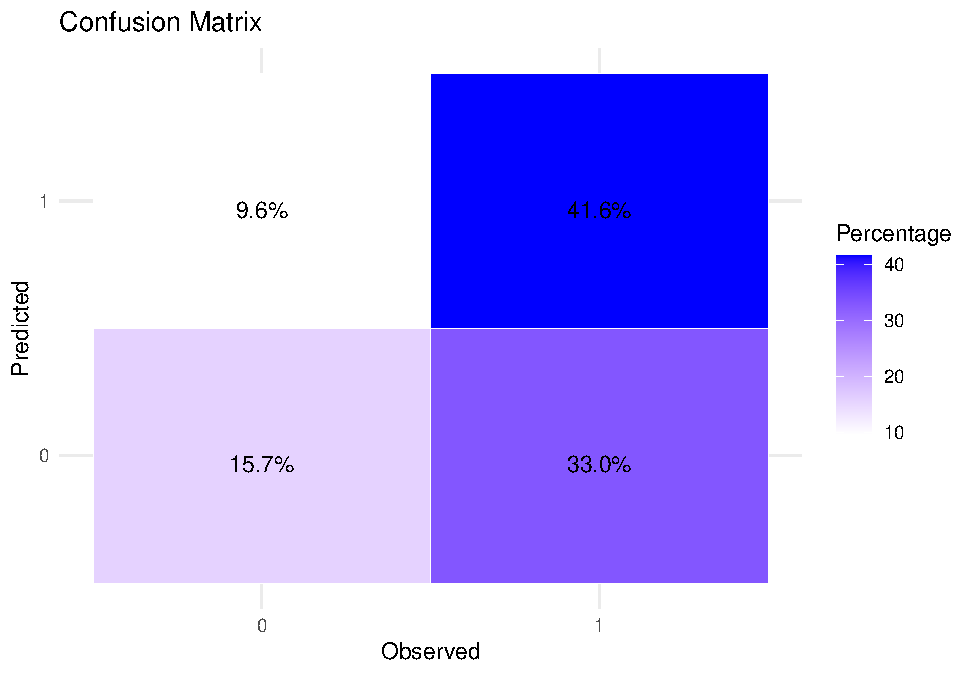
\includegraphics{Project-6-Morales_files/figure-latex/unnamed-chunk-5-1.pdf}

\begin{Shaded}
\begin{Highlighting}[]
\CommentTok{\# 10 random covariate balance plots (hint try gridExtra)}


\FunctionTok{set.seed}\NormalTok{(}\DecValTok{456}\NormalTok{) }
\NormalTok{selected\_indices }\OtherTok{\textless{}{-}} \FunctionTok{sample}\NormalTok{(}\FunctionTok{length}\NormalTok{(results), }\DecValTok{10}\NormalTok{)}
\NormalTok{selected\_models }\OtherTok{\textless{}{-}}\NormalTok{ results[selected\_indices]}

\FunctionTok{library}\NormalTok{(gridExtra)}
\end{Highlighting}
\end{Shaded}

\begin{verbatim}
## 
## Attaching package: 'gridExtra'
\end{verbatim}

\begin{verbatim}
## The following object is masked from 'package:dplyr':
## 
##     combine
\end{verbatim}

\begin{Shaded}
\begin{Highlighting}[]
\NormalTok{plot\_list }\OtherTok{\textless{}{-}} \FunctionTok{lapply}\NormalTok{(selected\_models, }\ControlFlowTok{function}\NormalTok{(model) \{}
  \CommentTok{\# Extract the matchit object}
\NormalTok{  matchit\_obj }\OtherTok{\textless{}{-}}\NormalTok{ model}\SpecialCharTok{$}\NormalTok{model}
  
  \CommentTok{\# Create the Love plot}
\NormalTok{  p }\OtherTok{\textless{}{-}} \FunctionTok{love.plot}\NormalTok{(matchit\_obj, }\AttributeTok{print =} \ConstantTok{FALSE}\NormalTok{, }\AttributeTok{drop.distance =} \ConstantTok{TRUE}\NormalTok{, }\AttributeTok{thresholds =} \FunctionTok{c}\NormalTok{(}\AttributeTok{m =} \FloatTok{0.1}\NormalTok{))  }
  \FunctionTok{return}\NormalTok{(p)}
\NormalTok{\})}

\CommentTok{\# Arrange the plots in a grid}
\FunctionTok{grid.arrange}\NormalTok{(}\AttributeTok{grobs =}\NormalTok{ plot\_list, }\AttributeTok{ncol =} \DecValTok{2}\NormalTok{)}
\end{Highlighting}
\end{Shaded}

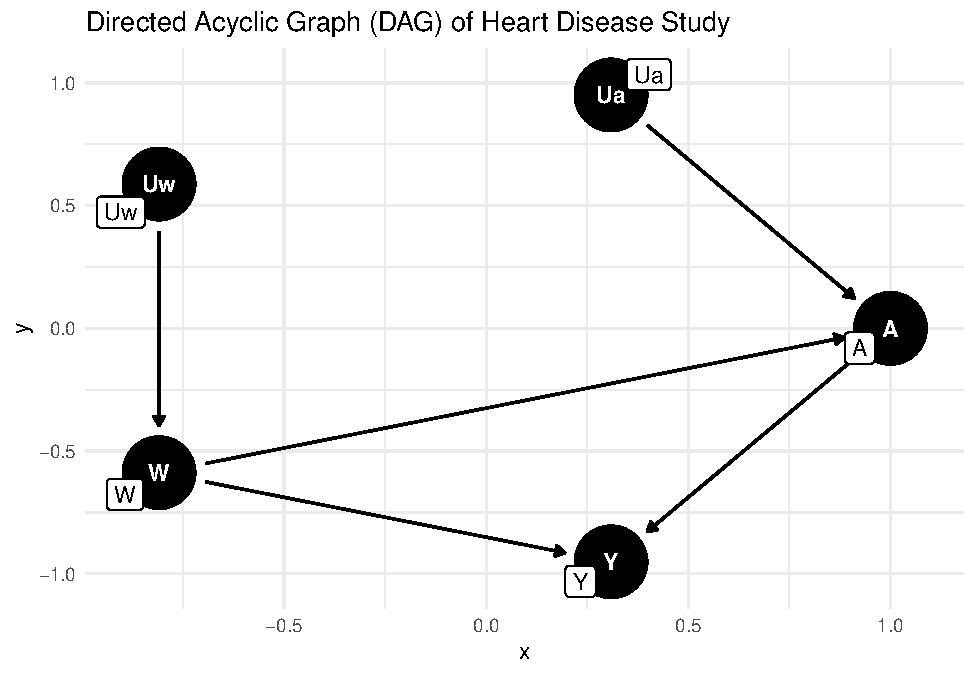
\includegraphics{Project-6-Morales_files/figure-latex/unnamed-chunk-6-1.pdf}

\begin{Shaded}
\begin{Highlighting}[]
\CommentTok{\# Note: ggplot objects are finnicky so ask for help if you\textquotesingle{}re struggling to automatically create them; consider using functions!}
\end{Highlighting}
\end{Shaded}

\hypertarget{questions-1}{%
\subsection{Questions}\label{questions-1}}

\begin{enumerate}
    \item \textbf{How many simulations resulted in models with a higher proportion of balanced covariates? Do you have any concerns about this?}
    Your Answer: In the first model we had $32/55=58\%$ of balanced covariates, in the simulations it was 40% 
    \item \textbf{Analyze the distribution of the ATTs. Do you have any concerns about this distribution?}
    Your Answer:Yes, the ATT increases as the percentage of balanced covariates increases, which can make the model results very weak to specifications of the matching that lead to different covariate balances. 
    \item \textbf{Do your 10 randomly chosen covariate balance plots produce similar numbers on the same covariates? Is it a concern if they do not?}
    Your Answer:It is not easy to see, but honestly I expect that this might change a lot depending of the inclusion of the variables, and specifications. Again this aligns with the idea that psm is prone to mispecification.  
\end{enumerate}

\hypertarget{matching-algorithm-of-your-choice}{%
\section{Matching Algorithm of Your
Choice}\label{matching-algorithm-of-your-choice}}

\hypertarget{simulate-alternative-model}{%
\subsection{Simulate Alternative
Model}\label{simulate-alternative-model}}

Henderson/Chatfield propose using genetic matching to learn the best
weights for Mahalanobis distance matching. Choose a matching algorithm
other than the propensity score (you may use genetic matching if you
wish, but it is also fine to use the greedy or optimal algorithms we
covered in lab instead). Repeat the same steps as specified in Section
4.2 and answer the following questions:

\begin{Shaded}
\begin{Highlighting}[]
\CommentTok{\#alternative model }

\CommentTok{\# I will also remove interview id and rows that have missing variables }
\NormalTok{baseline\_vars }\OtherTok{\textless{}{-}} \FunctionTok{colnames}\NormalTok{(ypsps)[}\SpecialCharTok{!}\FunctionTok{grepl}\NormalTok{(}\StringTok{"1973"}\NormalTok{, }\FunctionTok{colnames}\NormalTok{(ypsps)) }\SpecialCharTok{\&}
                                 \SpecialCharTok{!}\FunctionTok{grepl}\NormalTok{(}\StringTok{"1982"}\NormalTok{, }\FunctionTok{colnames}\NormalTok{(ypsps)) }\SpecialCharTok{\&}
                                 \FunctionTok{colnames}\NormalTok{(ypsps) }\SpecialCharTok{!=} \StringTok{"interviewid"} \SpecialCharTok{\&}
                                 \FunctionTok{colnames}\NormalTok{(ypsps) }\SpecialCharTok{!=} \StringTok{"student\_ppnscal"}\NormalTok{]}

\CommentTok{\# Remove rows with missing values in the selected columns}
\NormalTok{ypsps\_clean }\OtherTok{\textless{}{-}}\NormalTok{ ypsps[}\FunctionTok{complete.cases}\NormalTok{(ypsps[, baseline\_vars]), ]}


\CommentTok{\# Print the filtered list of variable names}
\CommentTok{\#print(baseline\_vars)}

\CommentTok{\# I will comment all to avoid running all again . }
\CommentTok{\# Randomly select features}

\CommentTok{\#set.seed(546)  }

\CommentTok{\# It tried running a 1000, it was too much. I stopped the code at 198. Ill do the analysis with that. }
\CommentTok{\#n\_iterations \textless{}{-} 198}
\CommentTok{\#data\_simulation2 \textless{}{-} data.frame(run\_id = integer(),}
                        \CommentTok{\#      n\_covar = integer(),}
                        \CommentTok{\#      ATT = double(),}
                        \CommentTok{\#      pct\_balanced = double(),}
                         \CommentTok{\#     mean\_pct\_impr = double())}



\CommentTok{\#for (i in 1:n\_iterations) \{}
  \CommentTok{\# Randomly select a number of variables from baseline\_vars}
 \CommentTok{\# n\_vars \textless{}{-} sample(1:length(baseline\_vars), 1)}
 \CommentTok{\# selected\_vars \textless{}{-} sample(baseline\_vars, n\_vars)}

  \CommentTok{\# Create and perform matching using selected\_vars}
  \CommentTok{\#formula\_str \textless{}{-} paste("college \textasciitilde{}", paste(selected\_vars, collapse = " + "))}
  \CommentTok{\#formula \textless{}{-} as.formula(formula\_str)}
  \CommentTok{\#matchit\_res2 \textless{}{-} matchit(formula, data = ypsps\_clean, method = "genetic" , }
                  \CommentTok{\#       distance = "glm",\# use glm, which by default is logistic regression}
                    \CommentTok{\#     link = "logit",\# specify we want a logit model, default when distance is specified}
                    \CommentTok{\#     estimand="ATT",}
                    \CommentTok{\#     discard = "none",\# obs to be discarded that are outside region of common support}
                         \CommentTok{\# whether matching should be done with replacement}
                     \CommentTok{\#    ratio = 1)}

  \CommentTok{\# Estimate ATT using linear regression on the matched data}
 \CommentTok{\# matched\_data2 \textless{}{-} match.data(matchit\_res2)}
 \CommentTok{\# lm\_formula \textless{}{-} as.formula(paste("student\_ppnscal \textasciitilde{} college +", paste(selected\_vars, collapse = " + ")))}
  \CommentTok{\#att\_model2 \textless{}{-} lm(lm\_formula, data = matched\_data2, weights=weights)}
  \CommentTok{\#att2 \textless{}{-} coef(summary(att\_model2))["college", "Estimate"]}

  
  \CommentTok{\# Calculate the proportion of covariates with SMD ≤ 0.1 and mean percent improvement in SMD}
  \CommentTok{\#balance2\textless{}{-} bal.tab(matchit\_res2 , binary="std", m.threshold=0.1 )}
 \CommentTok{\# df\_balance2 \textless{}{-} as.data.frame(balance2$Balance$M.Threshold)}
  
\CommentTok{\#  n\_total2 \textless{}{-} nrow(df\_balance2)}
 \CommentTok{\# n\_balanced2 \textless{}{-} length(df\_balance2[which(balance2$Balance$M.Threshold == "Balanced, \textless{}0.1"),])}
 \CommentTok{\# pct\_balanced2 \textless{}{-} (n\_balanced2/n\_total2)}
  

\CommentTok{\#matchit\_summary2 \textless{}{-} summary(matchit\_res2, improvement = TRUE)}

\CommentTok{\# Extract the reduction in standardized mean differences}
\CommentTok{\#improvement\_data2 \textless{}{-} matchit\_summary2$reduction}

\CommentTok{\# Specifically, if you\textquotesingle{}re interested in the reduction of SMDs}
\CommentTok{\#smd\_reduction2 \textless{}{-} improvement\_data2[,"Std. Mean Diff."]}

\CommentTok{\# You can calculate the mean percent improvement if needed}
\CommentTok{\#mean\_percent\_improvement2 \textless{}{-} mean(smd\_reduction2, na.rm = TRUE)}



  \CommentTok{\# put all this into a dataframe}
\CommentTok{\#  data\_sim2 \textless{}{-} data.frame(run\_id = i,}
 \CommentTok{\#                         n\_covar = n\_vars,}
 \CommentTok{\#                         ATT = att2,}
 \CommentTok{\#                         pct\_balanced2 = pct\_balanced2, }
 \CommentTok{\#                         mean\_pct\_impr2=mean\_percent\_improvement2)}

\CommentTok{\#  data\_simulation2 \textless{}{-} rbind(data\_simulation2, data\_sim2)}

\CommentTok{\#\}}
\end{Highlighting}
\end{Shaded}

\begin{Shaded}
\begin{Highlighting}[]
\CommentTok{\# Plot ATT v. proportion}

\CommentTok{\#graph\_genetic \textless{}{-} ggplot(data\_simulation2, aes(x =pct\_balanced2, y = ATT)) + }
 \CommentTok{\# geom\_point() +  \# Add points}
  \CommentTok{\#theme\_minimal() +  \# Use a minimal theme for aesthetics}
  \CommentTok{\#labs(x = "Percentage Balanced", y = "ATT", }
   \CommentTok{\#    title = "Scatter Plot of ATT vs. Percentage Balanced Genetic Matching")}
\CommentTok{\#graph\_genetic }
\CommentTok{\#ggsave("graph\_genetic.png", graph\_genetic, width = 6, height = 4)}
\end{Highlighting}
\end{Shaded}

\begin{figure}
\centering
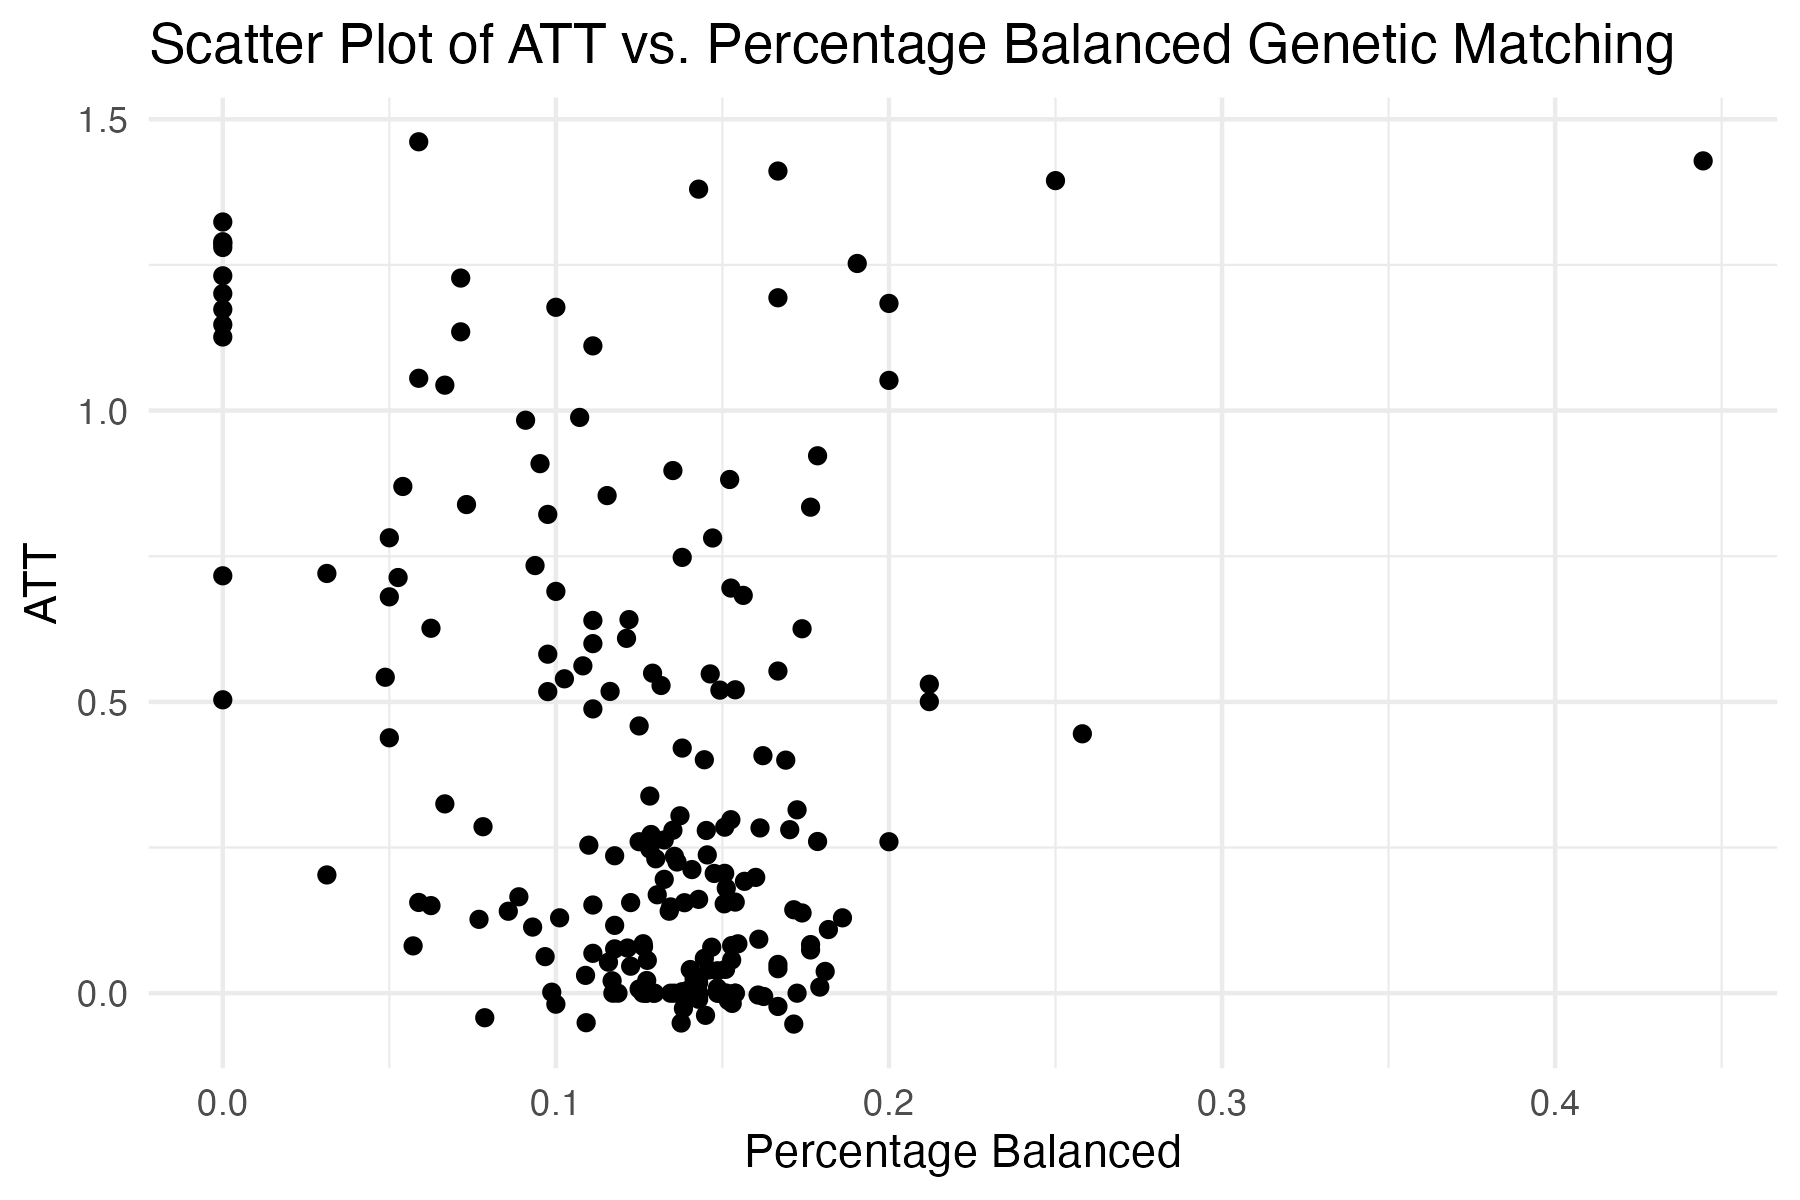
\includegraphics{graph_genetic.png}
\caption{GraphGen}
\end{figure}

\begin{Shaded}
\begin{Highlighting}[]
\CommentTok{\# Percentage balanced }
\CommentTok{\#mean\_pct\_bal\_genetic \textless{}{-} mean(data\_simulation2$pct\_balanced2)}
\CommentTok{\#mean\_pct\_bal\_nn \textless{}{-} mean(data\_simulation$pct\_balanced)}
\CommentTok{\#mean\_pct\_bal\_genetic}
\CommentTok{\#mean\_pct\_bal\_nn}
\end{Highlighting}
\end{Shaded}

\begin{Shaded}
\begin{Highlighting}[]
\CommentTok{\# Visualization for distributions of percent improvement}

\CommentTok{\#graph\_denisities \textless{}{-} ggplot() +}
 \CommentTok{\# geom\_density(data = data\_simulation, aes(x = mean\_pct\_impr, fill = "Propensity Score Model"), alpha = 0.5) +}
  \CommentTok{\#geom\_density(data = data\_simulation2, aes(x = mean\_pct\_impr2, fill = "Genetic"), alpha = 0.5) +}
  \CommentTok{\#labs(title = "Density Plot of Mean Percentage Improvement by Models", }
   \CommentTok{\#    x = "Mean Percentage Improvement", }
    \CommentTok{\# y = "Density") +}
  \CommentTok{\#scale\_fill\_manual(values = c("Propensity Score Model" = "blue", "Genetic" = "red")) +}
  \CommentTok{\#theme\_minimal() }
  
\CommentTok{\#ggsave("graph\_denisities.png", graph\_denisities, width = 6, height = 4)}
\end{Highlighting}
\end{Shaded}

\begin{figure}
\centering
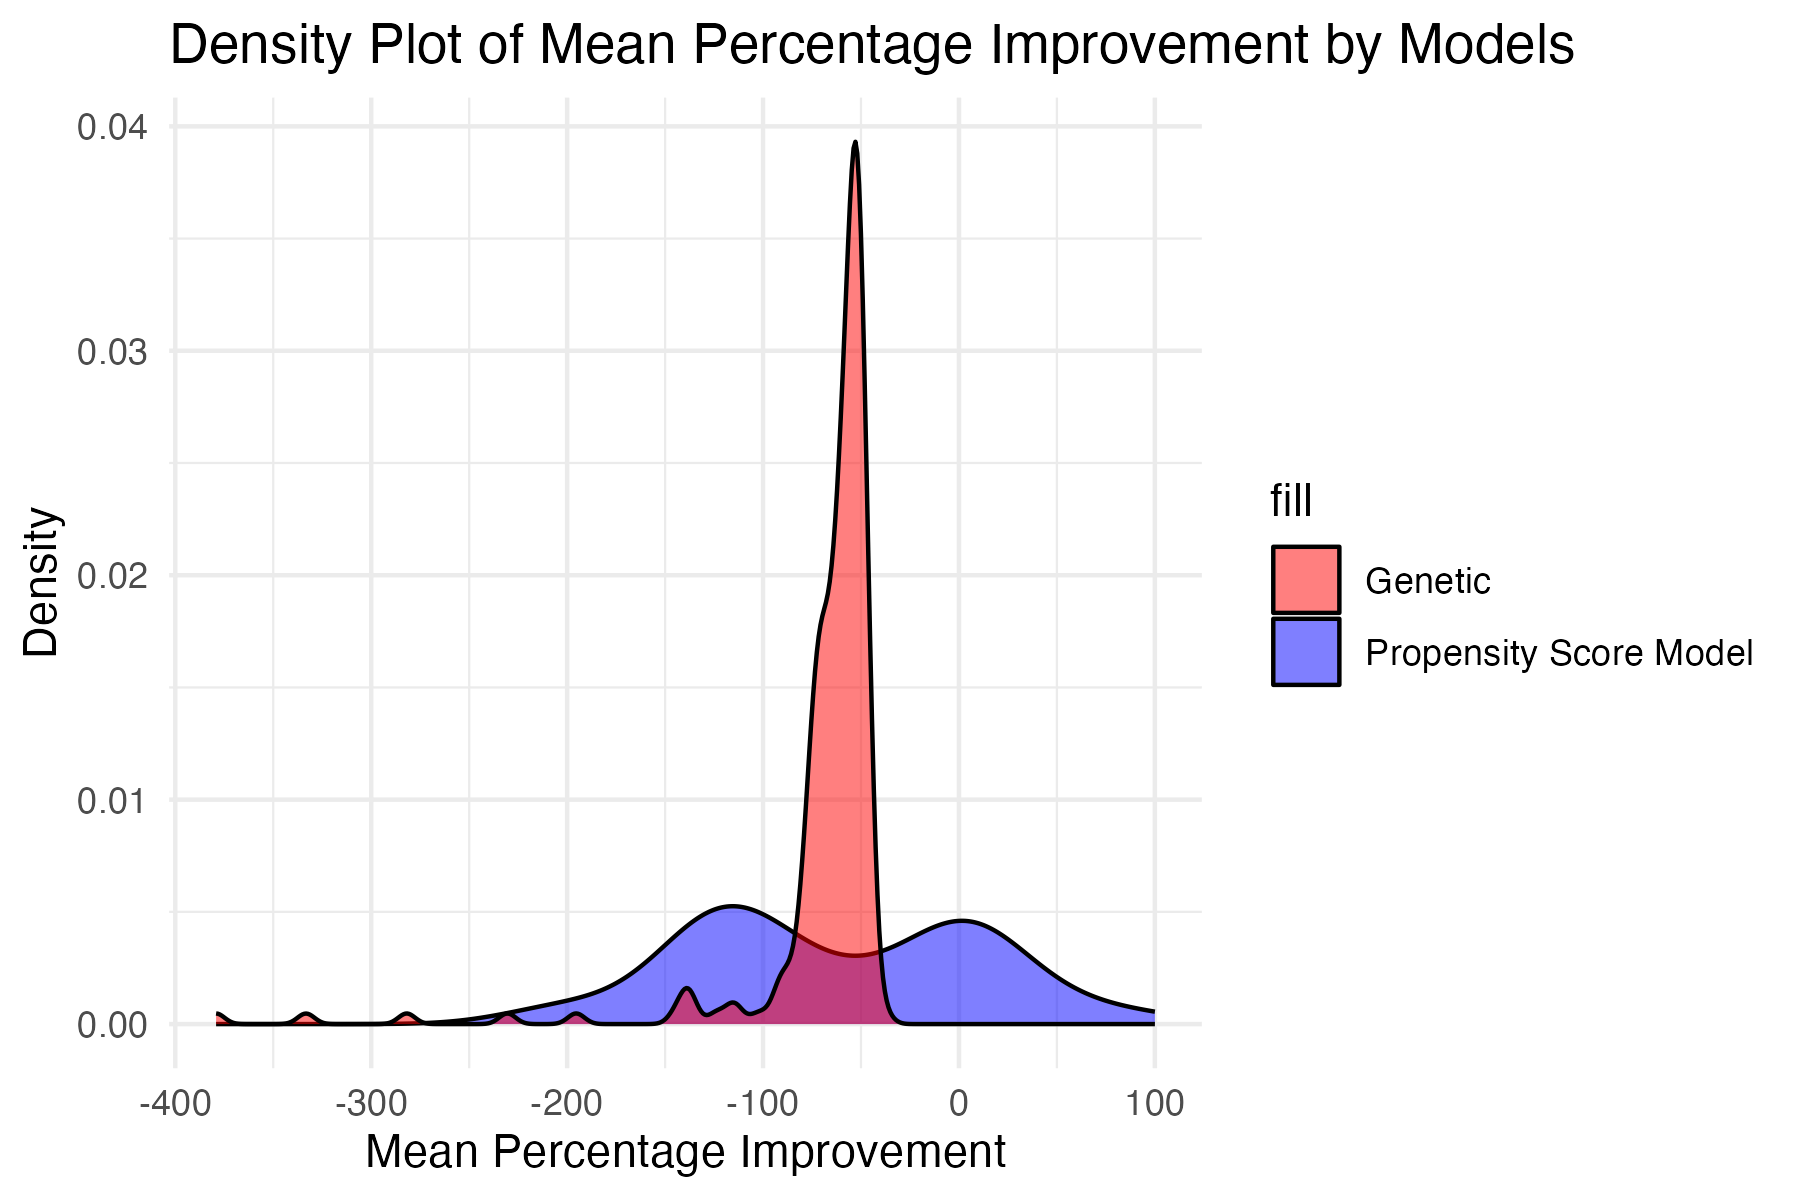
\includegraphics{graph_denisities.png}
\caption{GraphDensities}
\end{figure}

\hypertarget{questions-2}{%
\subsection{Questions}\label{questions-2}}

\begin{enumerate}
    \item \textbf{Does your alternative matching method have more runs with higher proportions of balanced covariates?}
     Your Answer:No, when I compared the averages of percentage covars balanced in each case, I found that the percentage is higher $(40\%)$ than the genetic case $(13\%)$ 
    \item \textbf{Use a visualization to examine the change in the distribution of the percent improvement in balance in propensity score matching vs. the distribution of the percent improvement in balance in your new method. Which did better? Analyze the results in 1-2 sentences.} 
    Your Answer: In the graph above we can see how the genetic one had a very narrowed distribution around $-60$ more or less, and then the original model, nearest neighbors is sparse with two modes, one in zero and one below $-100$. This is quite curious as I dont know exactly why. My intepretation is that at least the genetic one was making more improvements than the nn, because nn has many cases in 0 improvement and genetic doesnt. 
\end{enumerate}

\textbf{Optional:} Looking ahead to the discussion questions, you may
choose to model the propensity score using an algorithm other than
logistic regression and perform these simulations again, if you wish to
explore the second discussion question further.

\hypertarget{discussion-questions}{%
\subsection{Discussion Questions}\label{discussion-questions}}

\begin{enumerate}
    \item \textbf{Why might it be a good idea to do matching even if we have a randomized or as-if-random design?}
    Your Answer: There will be some cases in which the distribution of the covariables in each group might make the group substantially different, maybe in the randomization something happened, or by mere chance the groups were unbalanced. In that case Matching can help to solve any potential bias arising from substantially different distributions of covariables that might have an effect on the outcome. Importantly, this correction uses observable characteristics so it is also prone to biases, and could end up adding more bias. 
    \item \textbf{The standard way of estimating the propensity score is using a logistic regression to estimate probability of treatment. Given what we know about the curse of dimensionality, do you think there might be advantages to using other machine learning algorithms (decision trees, bagging/boosting forests, ensembles, etc.) to estimate propensity scores instead?}
    Your Answer:Yes, yes, and yes. That is what is behind TMLE for example. Using ensamble models we can find the best function to approximate the distribution or function of the treatment function, thus improving our chances to get the first stage of a doubly robust estimator correctly estimated. I think models that can reduce dimensions will improve matching. 
    
    
\end{enumerate}

\end{document}
